% Created 2017-12-11 Mon 15:57
% Intended LaTeX compiler: pdflatex
\documentclass{tufte-handout}
\usepackage[utf8]{inputenc}
\usepackage[T1]{fontenc}
\usepackage{graphicx}
\usepackage{grffile}
\usepackage{longtable}
\usepackage{wrapfig}
\usepackage{rotating}
\usepackage[normalem]{ulem}
\usepackage{amsmath}
\usepackage{textcomp}
\usepackage{amssymb}
\usepackage{capt-of}
\usepackage{hyperref}
\usepackage{graphicx} % allow embedded images
\setkeys{Gin}{width=\linewidth,totalheight=\textheight,keepaspectratio}
\graphicspath{{graphics/}} % set of paths to search for images
\usepackage{amsmath}  % extended mathematics
\usepackage{booktabs} % book-quality tables
\usepackage{units}    % non-stacked fractions and better unit spacing
\usepackage{multicol} % multiple column layout facilities
\usepackage{lipsum}   % filler text
\usepackage{fancyvrb} % extended verbatim environments
\fvset{fontsize=\normalsize}% default font size for fancy-verbatim environments
\usepackage{cancel}
\usepackage{cleveref}
\hypersetup{
colorlinks = true,
urlcolor = cyan}
\newcommand{\doccmd}[1]{\texttt{\textbackslash#1}}% command name -- adds backslash automatically
\newcommand{\docopt}[1]{\ensuremath{\langle}\textrm{\textit{#1}}\ensuremath{\rangle}}% optional command argument
\newcommand{\docarg}[1]{\textrm{\textit{#1}}}% (required) command argument
\newcommand{\docenv}[1]{\textsf{#1}}% environment name
\newcommand{\docpkg}[1]{\texttt{#1}}% package name
\newcommand{\doccls}[1]{\texttt{#1}}% document class name
\newcommand{\docclsopt}[1]{\texttt{#1}}% document class option name
\newenvironment{docspec}{\begin{quote}\noindent}{\end{quote}}% command specification environment
% Zach del Rosario's LaTeX macros (zdelrosario@outlook.com)
% Inspired by Paul Constantine, Art Owen
% Thanks to David Carlisle for writing the numdef package,
%    which makes the fraction definitions possible!

% Use % Zach del Rosario's LaTeX macros (zdelrosario@outlook.com)
% Inspired by Paul Constantine, Art Owen
% Thanks to David Carlisle for writing the numdef package,
%    which makes the fraction definitions possible!

% Use % Zach del Rosario's LaTeX macros (zdelrosario@outlook.com)
% Inspired by Paul Constantine, Art Owen
% Thanks to David Carlisle for writing the numdef package,
%    which makes the fraction definitions possible!

% Use \input{zachs_macros} in preamble of a latex document

% --------------------------------------------------
% Use some package dependencies
% --------------------------------------------------
\usepackage{amsmath}  % for \boldsymbol, etc.
\usepackage{amsfonts} % for \mathbb, etc.
\usepackage{scalerel,stackengine} % for \reallywidehat{}
\usepackage{graphicx} % for \includegraphics
\usepackage{caption}  % for captioning
\usepackage{mathtools}% for \ceil and \floor
\usepackage{forest}   % for forest environment

% --------------------------------------------------
% Figures and tables
% --------------------------------------------------
% Could use as-is; better for pattern matching

% Image Macro: \img{filename}{caption}
\newcommand{\img}[2]{
	\begin{figure}[H]
	\centering
	\includegraphics[width=0.6\textwidth]{../images/#1}   % first argument is the file
	\caption{#2}                  % second argument is caption
	\label{fig:#1}                % generate label from first argument
	\end{figure} }

% Double Image Macro: \img{file1}{file2}{caption1}{caption2}
\newcommand{\imgtwo}[4]{
	\begin{figure}
	\centering
	\begin{minipage}{.5\textwidth}
		\centering
		\includegraphics[width=0.9\linewidth]{../images/#1}
		\captionof{figure}{#3}
		\label{fig:#1}
	\end{minipage}%
	\begin{minipage}{.5\textwidth}
		\centering
		\includegraphics[width=0.9\linewidth]{../images/#2}
		\captionof{figure}{#4}
		\label{fig:#2}
	\end{minipage}
	\end{figure}
}

% Table Macro: \tab{filename}{caption}
\newcommand{\tab}[2]{
	\begin{table}[H]
	\centering
	\input{#1} 	% first argument is filename
	\caption{#2} 			% second argument is caption
	\label{tab:#1} 			% generate label from filename
	\end{table}
}

% --------------------------------------------------
% Common sets
% --------------------------------------------------
% Lovingly ripped from Art Owen
\def\reals{\mathbb{R}} % Real number symbol
\def\integers{\mathbb{Z}} % Integer symbol
\def\rationals{\mathbb{Q}} % Rational numbers
\def\naturals{\mathbb{N}} % Natural numbers
\def\complex{\mathbb{C}} % Complex numbers
% With exponent
\def\R#1{\mathbb{R}^{#1}}
\def\Z#1{\mathbb{Z}^{#1}}
\def\Q#1{\mathbb{Q}^{#1}}
\def\N#1{\mathbb{N}^{#1}}
\def\C#1{\mathbb{C}^{#1}}

% --------------------------------------------------
% Vectors and Matrices
% --------------------------------------------------
% Vector symbol macros
\newcommand{\vsym}[1]{\boldsymbol{#1}}
\def\v#1{\vsym{#1}} % \v{x} for vector symbol
% Quick letter vectors
\newcommand{\va}{\boldsymbol{a}}
\newcommand{\vb}{\boldsymbol{b}}
\newcommand{\vc}{\boldsymbol{c}}
\newcommand{\vd}{\boldsymbol{d}}
\newcommand{\ve}{\boldsymbol{e}}
\newcommand{\vf}{\boldsymbol{f}}
\newcommand{\vg}{\boldsymbol{g}}
\newcommand{\vh}{\boldsymbol{h}}
\newcommand{\vi}{\boldsymbol{i}}
\newcommand{\vj}{\boldsymbol{j}}
\newcommand{\vk}{\boldsymbol{k}}
\newcommand{\vl}{\boldsymbol{l}}
\newcommand{\vm}{\boldsymbol{m}}
\newcommand{\vn}{\boldsymbol{n}}
\newcommand{\vo}{\boldsymbol{o}}
\newcommand{\vp}{\boldsymbol{p}}
\newcommand{\vq}{\boldsymbol{q}}
\newcommand{\vr}{\boldsymbol{r}}
\newcommand{\vs}{\boldsymbol{s}}
\newcommand{\vt}{\boldsymbol{t}}
\newcommand{\vu}{\boldsymbol{u}}
\newcommand{\vv}{\boldsymbol{v}}
\newcommand{\vw}{\boldsymbol{w}}
\newcommand{\vx}{\boldsymbol{x}}
\newcommand{\vy}{\boldsymbol{y}}
\newcommand{\vz}{\boldsymbol{z}}

% Tilde shortcut
\newcommand{\tl}[1]{\tilde{#1}}
% Vector symbol + tilde macros
\newcommand{\vta}{\tilde{\boldsymbol{a}}}
\newcommand{\vtb}{\tilde{\boldsymbol{b}}}
\newcommand{\vtc}{\tilde{\boldsymbol{c}}}
\newcommand{\vtd}{\tilde{\boldsymbol{d}}}
\newcommand{\vte}{\tilde{\boldsymbol{e}}}
\newcommand{\vtf}{\tilde{\boldsymbol{f}}}
\newcommand{\vtg}{\tilde{\boldsymbol{g}}}
\newcommand{\vth}{\tilde{\boldsymbol{h}}}
\newcommand{\vti}{\tilde{\boldsymbol{i}}}
\newcommand{\vtj}{\tilde{\boldsymbol{j}}}
\newcommand{\vtk}{\tilde{\boldsymbol{k}}}
\newcommand{\vtl}{\tilde{\boldsymbol{l}}}
\newcommand{\vtm}{\tilde{\boldsymbol{m}}}
\newcommand{\vtn}{\tilde{\boldsymbol{n}}}
\newcommand{\vto}{\tilde{\boldsymbol{o}}}
\newcommand{\vtp}{\tilde{\boldsymbol{p}}}
\newcommand{\vtq}{\tilde{\boldsymbol{q}}}
\newcommand{\vtr}{\tilde{\boldsymbol{r}}}
\newcommand{\vts}{\tilde{\boldsymbol{s}}}
\newcommand{\vtt}{\tilde{\boldsymbol{t}}}
\newcommand{\vtu}{\tilde{\boldsymbol{u}}}
\newcommand{\vtv}{\tilde{\boldsymbol{v}}}
\newcommand{\vtw}{\tilde{\boldsymbol{w}}}
\newcommand{\vtx}{\tilde{\boldsymbol{x}}}
\newcommand{\vty}{\tilde{\boldsymbol{y}}}
\newcommand{\vtz}{\tilde{\boldsymbol{z}}}

% Vector symbol + hat macros
\newcommand{\vha}{\hat{\boldsymbol{a}}}
\newcommand{\vhb}{\hat{\boldsymbol{b}}}
\newcommand{\vhc}{\hat{\boldsymbol{c}}}
\newcommand{\vhd}{\hat{\boldsymbol{d}}}
\newcommand{\vhe}{\hat{\boldsymbol{e}}}
\newcommand{\vhf}{\hat{\boldsymbol{f}}}
\newcommand{\vhg}{\hat{\boldsymbol{g}}}
\newcommand{\vhh}{\hat{\boldsymbol{h}}}
\newcommand{\vhi}{\hat{\boldsymbol{i}}}
\newcommand{\vhj}{\hat{\boldsymbol{j}}}
\newcommand{\vhk}{\hat{\boldsymbol{k}}}
\newcommand{\vhl}{\hat{\boldsymbol{l}}}
\newcommand{\vhm}{\hat{\boldsymbol{m}}}
\newcommand{\vhn}{\hat{\boldsymbol{n}}}
\newcommand{\vho}{\hat{\boldsymbol{o}}}
\newcommand{\vhp}{\hat{\boldsymbol{p}}}
\newcommand{\vhq}{\hat{\boldsymbol{q}}}
\newcommand{\vhr}{\hat{\boldsymbol{r}}}
\newcommand{\vhs}{\hat{\boldsymbol{s}}}
\newcommand{\vht}{\hat{\boldsymbol{t}}}
\newcommand{\vhu}{\hat{\boldsymbol{u}}}
\newcommand{\vhv}{\hat{\boldsymbol{v}}}
\newcommand{\vhw}{\hat{\boldsymbol{w}}}
\newcommand{\vhx}{\hat{\boldsymbol{x}}}
\newcommand{\vhy}{\hat{\boldsymbol{y}}}
\newcommand{\vhz}{\hat{\boldsymbol{z}}}

% Matrix symbol
\newcommand{\msym}[1]{\boldsymbol{#1}}
\def\m#1{\msym{#1}} % short-shortcut

\newcommand{\mA}{\boldsymbol{A}}
\newcommand{\mB}{\boldsymbol{B}}
\newcommand{\mC}{\boldsymbol{C}}
\newcommand{\mD}{\boldsymbol{D}}
\newcommand{\mE}{\boldsymbol{E}}
\newcommand{\mF}{\boldsymbol{F}}
\newcommand{\mG}{\boldsymbol{G}}
\newcommand{\mH}{\boldsymbol{H}}
\newcommand{\mI}{\boldsymbol{I}}
\newcommand{\mJ}{\boldsymbol{J}}
\newcommand{\mK}{\boldsymbol{K}}
\newcommand{\mL}{\boldsymbol{L}}
\newcommand{\mM}{\boldsymbol{M}}
\newcommand{\mN}{\boldsymbol{N}}
\newcommand{\mO}{\boldsymbol{O}}
\newcommand{\mP}{\boldsymbol{P}}
\newcommand{\mQ}{\boldsymbol{Q}}
\newcommand{\mR}{\boldsymbol{R}}
\newcommand{\mS}{\boldsymbol{S}}
\newcommand{\mT}{\boldsymbol{T}}
\newcommand{\mU}{\boldsymbol{U}}
\newcommand{\mV}{\boldsymbol{V}}
\newcommand{\mW}{\boldsymbol{W}}
\newcommand{\mX}{\boldsymbol{X}}
\newcommand{\mY}{\boldsymbol{Y}}
\newcommand{\mZ}{\boldsymbol{Z}}

% Tilde over letter
\newcommand{\tla}{\tilde{a}}
\newcommand{\tlb}{\tilde{b}}
\newcommand{\tlc}{\tilde{c}}
\newcommand{\tld}{\tilde{d}}
\newcommand{\tle}{\tilde{e}}
\newcommand{\tlf}{\tilde{f}}
\newcommand{\tlg}{\tilde{g}}
\newcommand{\tlh}{\tilde{h}}
\newcommand{\tli}{\tilde{i}}
\newcommand{\tlj}{\tilde{j}}
\newcommand{\tlk}{\tilde{k}}
\newcommand{\tll}{\tilde{l}}
\newcommand{\tlm}{\tilde{m}}
\newcommand{\tln}{\tilde{n}}
\newcommand{\tlo}{\tilde{o}}
\newcommand{\tlp}{\tilde{p}}
\newcommand{\tlq}{\tilde{q}}
\newcommand{\tlr}{\tilde{r}}
\newcommand{\tls}{\tilde{s}}
\newcommand{\tlt}{\tilde{t}}
\newcommand{\tlu}{\tilde{u}}
\newcommand{\tlv}{\tilde{v}}
\newcommand{\tlw}{\tilde{w}}
\newcommand{\tlx}{\tilde{x}}
\newcommand{\tly}{\tilde{y}}
\newcommand{\tlz}{\tilde{z}}

% Caligraphic symbol
\def\c#1{\mathcal{#1}} % short-shortcut

\newcommand{\cA}{\mathcal{A}}
\newcommand{\cB}{\mathcal{B}}
\newcommand{\cC}{\mathcal{C}}
\newcommand{\cD}{\mathcal{D}}
\newcommand{\cE}{\mathcal{E}}
\newcommand{\cF}{\mathcal{F}}
\newcommand{\cG}{\mathcal{G}}
\newcommand{\cH}{\mathcal{H}}
\newcommand{\cI}{\mathcal{I}}
\newcommand{\cJ}{\mathcal{J}}
\newcommand{\cK}{\mathcal{K}}
\newcommand{\cL}{\mathcal{L}}
\newcommand{\cM}{\mathcal{M}}
\newcommand{\cN}{\mathcal{N}}
\newcommand{\cO}{\mathcal{O}}
\newcommand{\cP}{\mathcal{P}}
\newcommand{\cQ}{\mathcal{Q}}
\newcommand{\cR}{\mathcal{R}}
\newcommand{\cS}{\mathcal{S}}
\newcommand{\cT}{\mathcal{T}}
\newcommand{\cU}{\mathcal{U}}
\newcommand{\cV}{\mathcal{V}}
\newcommand{\cW}{\mathcal{W}}
\newcommand{\cX}{\mathcal{X}}
\newcommand{\cY}{\mathcal{Y}}
\newcommand{\cZ}{\mathcal{Z}}
% --------------------------------------------------
% Common probability symbols
% --------------------------------------------------
% Lovingly ripped from Art Owen
\newcommand{\mrm}{\mathrm}
\def\E{\mathbb{E}} % Expectation symbol
\def\Earg#1{\E\left[{#1}\right]}
\def\Esubarg#1#2{\E_{#1}\left[{#2}\right]}
\def\P{\mathbb{P}} % Probability symbol
\def\Parg#1{\P\left({#1}\right)}
\def\Psubarg#1#2{\P_{#1}\left[{#2}\right]}
\def\Cov{\mrm{Cov}} % Covariance symbol
\def\Covarg#1{\Cov\left[{#1}\right]}
\def\Covsubarg#1#2{\Cov_{#1}\left[{#2}\right]}
\newcommand{\family}{\mathcal{P}} % probability family / statistical model
\newcommand{\iid}{\stackrel{\mathrm{iid}}{\sim}}
\newcommand{\ind}{\stackrel{\mathrm{ind}}{\sim}}
\def\V{\mathrm{V}} % Variance symbol

% --------------------------------------------------
% Misc
% --------------------------------------------------
% Angle bracket average
\newcommand{\avg}[1]{\left\langle#1\right\rangle}

% Floor and ceiling
% http://tex.stackexchange.com/questions/118173/how-to-write-ceil-and-floor-in-latex
\DeclarePairedDelimiter\ceil{\lceil}{\rceil}
\DeclarePairedDelimiter\floor{\lfloor}{\rfloor}

% Comical & useful reallywidehat
\stackMath
\newcommand\reallywidehat[1]{%
\savestack{\tmpbox}{\stretchto{%
  \scaleto{%
    \scalerel*[\widthof{\ensuremath{#1}}]{\kern-.6pt\bigwedge\kern-.6pt}%
    {\rule[-\textheight/2]{1ex}{\textheight}}%WIDTH-LIMITED BIG WEDGE
  }{\textheight}%
}{0.5ex}}%
\stackon[1pt]{#1}{\tmpbox}%
}

% Comical & useful reallywideparen
\newcommand\reallywideparen[1]{%
\begin{array}{c}
\stretchto{
  \scaleto{
    \scalerel*[\widthof{#1}]{\frown}
    {\rule[-\textheight/2]{1ex}{\textheight}} %WIDTH-LIMITED BIG WEDGE
  }{1.25\textheight} % THIS STRETCHES THE WEDGE A LITTLE EXTRA WIDE
}{0.5ex}\\           % THIS SQUEEZES THE WEDGE TO 0.5ex HEIGHT
#1\\                   % THIS STACKS THE WEDGE ATOP THE ARGUMENT
\rule{0ex}{.01ex}
\end{array}
}
% Useful for debugging; prints to document whether command has been defined already
% Via: http://tex.stackexchange.com/questions/30483/how-can-i-check-in-latex-or-plain-tex-whether-a-command-exists-by-name
\newcommand{\checkfor}[1]{%
  \ifcsname#1\endcsname%
    ... command '#1' exists ...%
  \else%
    ... command '#1' does not exist ...%
  \fi%
}

% Use a forest environment to depict a directory tree
% https://tex.stackexchange.com/questions/5073/making-a-simple-directory-tree
\newcommand{\ftree}[1]{%
\begin{forest}
for tree={
    font=\ttfamily,
    grow'=0,
    child anchor=west,
    parent anchor=south,
    anchor=west,
    calign=first,
    edge path={
      \noexpand\path [draw, \forestoption{edge}]
      (!u.south west) +(7.5pt,0) |- node[fill,inner sep=1.25pt] {} (.child anchor)\forestoption{edge label};
    },
    before typesetting nodes={
      if n=1
        {insert before={[,phantom]}}
        {}
    },
    fit=band,
    before computing xy={l=15pt},
  }%
  #1%
\end{forest}
}

% --------------------------------------------------
% Fractions
% --------------------------------------------------
\usepackage{numdef}   % prefixing with \num allows numbers at end of \newcommand name
\num\newcommand{\f12}{\frac{1}{2}}
\num\newcommand{\f13}{\frac{1}{3}}
\num\newcommand{\f14}{\frac{1}{4}}
\num\newcommand{\f15}{\frac{1}{5}}
\num\newcommand{\f16}{\frac{1}{6}}
\num\newcommand{\f17}{\frac{1}{7}}
\num\newcommand{\f18}{\frac{1}{8}}
\num\newcommand{\f19}{\frac{1}{9}}

\num\newcommand{\f22}{\frac{2}{2}}
\num\newcommand{\f23}{\frac{2}{3}}
\num\newcommand{\f24}{\frac{2}{4}}
\num\newcommand{\f25}{\frac{2}{5}}
\num\newcommand{\f26}{\frac{2}{6}}
\num\newcommand{\f27}{\frac{2}{7}}
\num\newcommand{\f28}{\frac{2}{8}}
\num\newcommand{\f29}{\frac{2}{9}}

\num\newcommand{\f32}{\frac{3}{2}}
\num\newcommand{\f33}{\frac{3}{3}}
\num\newcommand{\f34}{\frac{3}{4}}
\num\newcommand{\f35}{\frac{3}{5}}
\num\newcommand{\f36}{\frac{3}{6}}
\num\newcommand{\f37}{\frac{3}{7}}
\num\newcommand{\f38}{\frac{3}{8}}
\num\newcommand{\f39}{\frac{3}{9}}

\num\newcommand{\f42}{\frac{4}{2}}
\num\newcommand{\f43}{\frac{4}{3}}
\num\newcommand{\f44}{\frac{4}{4}}
\num\newcommand{\f45}{\frac{4}{5}}
\num\newcommand{\f46}{\frac{4}{6}}
\num\newcommand{\f47}{\frac{4}{7}}
\num\newcommand{\f48}{\frac{4}{8}}
\num\newcommand{\f49}{\frac{4}{9}}

\num\newcommand{\f52}{\frac{5}{2}}
\num\newcommand{\f53}{\frac{5}{3}}
\num\newcommand{\f54}{\frac{5}{4}}
\num\newcommand{\f55}{\frac{5}{5}}
\num\newcommand{\f56}{\frac{5}{6}}
\num\newcommand{\f57}{\frac{5}{7}}
\num\newcommand{\f58}{\frac{5}{8}}
\num\newcommand{\f59}{\frac{5}{9}}

\num\newcommand{\f62}{\frac{6}{2}}
\num\newcommand{\f63}{\frac{6}{3}}
\num\newcommand{\f64}{\frac{6}{4}}
\num\newcommand{\f65}{\frac{6}{5}}
\num\newcommand{\f66}{\frac{6}{6}}
\num\newcommand{\f67}{\frac{6}{7}}
\num\newcommand{\f68}{\frac{6}{8}}
\num\newcommand{\f69}{\frac{6}{9}}

\num\newcommand{\f72}{\frac{7}{2}}
\num\newcommand{\f73}{\frac{7}{3}}
\num\newcommand{\f74}{\frac{7}{4}}
\num\newcommand{\f75}{\frac{7}{5}}
\num\newcommand{\f76}{\frac{7}{6}}
\num\newcommand{\f77}{\frac{7}{7}}
\num\newcommand{\f78}{\frac{7}{8}}
\num\newcommand{\f79}{\frac{7}{9}}

\num\newcommand{\f82}{\frac{8}{2}}
\num\newcommand{\f83}{\frac{8}{3}}
\num\newcommand{\f84}{\frac{8}{4}}
\num\newcommand{\f85}{\frac{8}{5}}
\num\newcommand{\f86}{\frac{8}{6}}
\num\newcommand{\f87}{\frac{8}{7}}
\num\newcommand{\f88}{\frac{8}{8}}
\num\newcommand{\f89}{\frac{8}{9}}

\num\newcommand{\f92}{\frac{9}{2}}
\num\newcommand{\f93}{\frac{9}{3}}
\num\newcommand{\f94}{\frac{9}{4}}
\num\newcommand{\f95}{\frac{9}{5}}
\num\newcommand{\f96}{\frac{9}{6}}
\num\newcommand{\f97}{\frac{9}{7}}
\num\newcommand{\f98}{\frac{9}{8}}
\num\newcommand{\f99}{\frac{9}{9}}

% --------------------------------------------------
% Cylindrical and Spherical operators
% --------------------------------------------------
% Cylindrical coordinates {r,\phi,z}
\num\newcommand{\cdiv1}[1]{\frac{1}{r}\frac{\partial}{\partial r}(r#1)}
\num\newcommand{\cdiv2}[1]{\frac{1}{r}\frac{\partial}{\partial\phi}(#1)}
\num\newcommand{\cdiv3}[1]{\frac{\partial}{\partial z}(#1)}

%--------------------------------------------------
% matminux
%--------------------------------------------------
% https://tex.stackexchange.com/questions/75545/negative-sign-and-matrix-alignment
\newcommand*{\mm}{%
  \leavevmode
  \hphantom{0}%
  \llap{%
    \settowidth{\dimen0 }{$0$}%
    \resizebox{1.1\dimen0 }{\height}{$-$}%
  }%
}
 in preamble of a latex document

% --------------------------------------------------
% Use some package dependencies
% --------------------------------------------------
\usepackage{amsmath}  % for \boldsymbol, etc.
\usepackage{amsfonts} % for \mathbb, etc.
\usepackage{scalerel,stackengine} % for \reallywidehat{}
\usepackage{graphicx} % for \includegraphics
\usepackage{caption}  % for captioning
\usepackage{mathtools}% for \ceil and \floor
\usepackage{forest}   % for forest environment

% --------------------------------------------------
% Figures and tables
% --------------------------------------------------
% Could use as-is; better for pattern matching

% Image Macro: \img{filename}{caption}
\newcommand{\img}[2]{
	\begin{figure}[H]
	\centering
	\includegraphics[width=0.6\textwidth]{../images/#1}   % first argument is the file
	\caption{#2}                  % second argument is caption
	\label{fig:#1}                % generate label from first argument
	\end{figure} }

% Double Image Macro: \img{file1}{file2}{caption1}{caption2}
\newcommand{\imgtwo}[4]{
	\begin{figure}
	\centering
	\begin{minipage}{.5\textwidth}
		\centering
		\includegraphics[width=0.9\linewidth]{../images/#1}
		\captionof{figure}{#3}
		\label{fig:#1}
	\end{minipage}%
	\begin{minipage}{.5\textwidth}
		\centering
		\includegraphics[width=0.9\linewidth]{../images/#2}
		\captionof{figure}{#4}
		\label{fig:#2}
	\end{minipage}
	\end{figure}
}

% Table Macro: \tab{filename}{caption}
\newcommand{\tab}[2]{
	\begin{table}[H]
	\centering
	\input{#1} 	% first argument is filename
	\caption{#2} 			% second argument is caption
	\label{tab:#1} 			% generate label from filename
	\end{table}
}

% --------------------------------------------------
% Common sets
% --------------------------------------------------
% Lovingly ripped from Art Owen
\def\reals{\mathbb{R}} % Real number symbol
\def\integers{\mathbb{Z}} % Integer symbol
\def\rationals{\mathbb{Q}} % Rational numbers
\def\naturals{\mathbb{N}} % Natural numbers
\def\complex{\mathbb{C}} % Complex numbers
% With exponent
\def\R#1{\mathbb{R}^{#1}}
\def\Z#1{\mathbb{Z}^{#1}}
\def\Q#1{\mathbb{Q}^{#1}}
\def\N#1{\mathbb{N}^{#1}}
\def\C#1{\mathbb{C}^{#1}}

% --------------------------------------------------
% Vectors and Matrices
% --------------------------------------------------
% Vector symbol macros
\newcommand{\vsym}[1]{\boldsymbol{#1}}
\def\v#1{\vsym{#1}} % \v{x} for vector symbol
% Quick letter vectors
\newcommand{\va}{\boldsymbol{a}}
\newcommand{\vb}{\boldsymbol{b}}
\newcommand{\vc}{\boldsymbol{c}}
\newcommand{\vd}{\boldsymbol{d}}
\newcommand{\ve}{\boldsymbol{e}}
\newcommand{\vf}{\boldsymbol{f}}
\newcommand{\vg}{\boldsymbol{g}}
\newcommand{\vh}{\boldsymbol{h}}
\newcommand{\vi}{\boldsymbol{i}}
\newcommand{\vj}{\boldsymbol{j}}
\newcommand{\vk}{\boldsymbol{k}}
\newcommand{\vl}{\boldsymbol{l}}
\newcommand{\vm}{\boldsymbol{m}}
\newcommand{\vn}{\boldsymbol{n}}
\newcommand{\vo}{\boldsymbol{o}}
\newcommand{\vp}{\boldsymbol{p}}
\newcommand{\vq}{\boldsymbol{q}}
\newcommand{\vr}{\boldsymbol{r}}
\newcommand{\vs}{\boldsymbol{s}}
\newcommand{\vt}{\boldsymbol{t}}
\newcommand{\vu}{\boldsymbol{u}}
\newcommand{\vv}{\boldsymbol{v}}
\newcommand{\vw}{\boldsymbol{w}}
\newcommand{\vx}{\boldsymbol{x}}
\newcommand{\vy}{\boldsymbol{y}}
\newcommand{\vz}{\boldsymbol{z}}

% Tilde shortcut
\newcommand{\tl}[1]{\tilde{#1}}
% Vector symbol + tilde macros
\newcommand{\vta}{\tilde{\boldsymbol{a}}}
\newcommand{\vtb}{\tilde{\boldsymbol{b}}}
\newcommand{\vtc}{\tilde{\boldsymbol{c}}}
\newcommand{\vtd}{\tilde{\boldsymbol{d}}}
\newcommand{\vte}{\tilde{\boldsymbol{e}}}
\newcommand{\vtf}{\tilde{\boldsymbol{f}}}
\newcommand{\vtg}{\tilde{\boldsymbol{g}}}
\newcommand{\vth}{\tilde{\boldsymbol{h}}}
\newcommand{\vti}{\tilde{\boldsymbol{i}}}
\newcommand{\vtj}{\tilde{\boldsymbol{j}}}
\newcommand{\vtk}{\tilde{\boldsymbol{k}}}
\newcommand{\vtl}{\tilde{\boldsymbol{l}}}
\newcommand{\vtm}{\tilde{\boldsymbol{m}}}
\newcommand{\vtn}{\tilde{\boldsymbol{n}}}
\newcommand{\vto}{\tilde{\boldsymbol{o}}}
\newcommand{\vtp}{\tilde{\boldsymbol{p}}}
\newcommand{\vtq}{\tilde{\boldsymbol{q}}}
\newcommand{\vtr}{\tilde{\boldsymbol{r}}}
\newcommand{\vts}{\tilde{\boldsymbol{s}}}
\newcommand{\vtt}{\tilde{\boldsymbol{t}}}
\newcommand{\vtu}{\tilde{\boldsymbol{u}}}
\newcommand{\vtv}{\tilde{\boldsymbol{v}}}
\newcommand{\vtw}{\tilde{\boldsymbol{w}}}
\newcommand{\vtx}{\tilde{\boldsymbol{x}}}
\newcommand{\vty}{\tilde{\boldsymbol{y}}}
\newcommand{\vtz}{\tilde{\boldsymbol{z}}}

% Vector symbol + hat macros
\newcommand{\vha}{\hat{\boldsymbol{a}}}
\newcommand{\vhb}{\hat{\boldsymbol{b}}}
\newcommand{\vhc}{\hat{\boldsymbol{c}}}
\newcommand{\vhd}{\hat{\boldsymbol{d}}}
\newcommand{\vhe}{\hat{\boldsymbol{e}}}
\newcommand{\vhf}{\hat{\boldsymbol{f}}}
\newcommand{\vhg}{\hat{\boldsymbol{g}}}
\newcommand{\vhh}{\hat{\boldsymbol{h}}}
\newcommand{\vhi}{\hat{\boldsymbol{i}}}
\newcommand{\vhj}{\hat{\boldsymbol{j}}}
\newcommand{\vhk}{\hat{\boldsymbol{k}}}
\newcommand{\vhl}{\hat{\boldsymbol{l}}}
\newcommand{\vhm}{\hat{\boldsymbol{m}}}
\newcommand{\vhn}{\hat{\boldsymbol{n}}}
\newcommand{\vho}{\hat{\boldsymbol{o}}}
\newcommand{\vhp}{\hat{\boldsymbol{p}}}
\newcommand{\vhq}{\hat{\boldsymbol{q}}}
\newcommand{\vhr}{\hat{\boldsymbol{r}}}
\newcommand{\vhs}{\hat{\boldsymbol{s}}}
\newcommand{\vht}{\hat{\boldsymbol{t}}}
\newcommand{\vhu}{\hat{\boldsymbol{u}}}
\newcommand{\vhv}{\hat{\boldsymbol{v}}}
\newcommand{\vhw}{\hat{\boldsymbol{w}}}
\newcommand{\vhx}{\hat{\boldsymbol{x}}}
\newcommand{\vhy}{\hat{\boldsymbol{y}}}
\newcommand{\vhz}{\hat{\boldsymbol{z}}}

% Matrix symbol
\newcommand{\msym}[1]{\boldsymbol{#1}}
\def\m#1{\msym{#1}} % short-shortcut

\newcommand{\mA}{\boldsymbol{A}}
\newcommand{\mB}{\boldsymbol{B}}
\newcommand{\mC}{\boldsymbol{C}}
\newcommand{\mD}{\boldsymbol{D}}
\newcommand{\mE}{\boldsymbol{E}}
\newcommand{\mF}{\boldsymbol{F}}
\newcommand{\mG}{\boldsymbol{G}}
\newcommand{\mH}{\boldsymbol{H}}
\newcommand{\mI}{\boldsymbol{I}}
\newcommand{\mJ}{\boldsymbol{J}}
\newcommand{\mK}{\boldsymbol{K}}
\newcommand{\mL}{\boldsymbol{L}}
\newcommand{\mM}{\boldsymbol{M}}
\newcommand{\mN}{\boldsymbol{N}}
\newcommand{\mO}{\boldsymbol{O}}
\newcommand{\mP}{\boldsymbol{P}}
\newcommand{\mQ}{\boldsymbol{Q}}
\newcommand{\mR}{\boldsymbol{R}}
\newcommand{\mS}{\boldsymbol{S}}
\newcommand{\mT}{\boldsymbol{T}}
\newcommand{\mU}{\boldsymbol{U}}
\newcommand{\mV}{\boldsymbol{V}}
\newcommand{\mW}{\boldsymbol{W}}
\newcommand{\mX}{\boldsymbol{X}}
\newcommand{\mY}{\boldsymbol{Y}}
\newcommand{\mZ}{\boldsymbol{Z}}

% Tilde over letter
\newcommand{\tla}{\tilde{a}}
\newcommand{\tlb}{\tilde{b}}
\newcommand{\tlc}{\tilde{c}}
\newcommand{\tld}{\tilde{d}}
\newcommand{\tle}{\tilde{e}}
\newcommand{\tlf}{\tilde{f}}
\newcommand{\tlg}{\tilde{g}}
\newcommand{\tlh}{\tilde{h}}
\newcommand{\tli}{\tilde{i}}
\newcommand{\tlj}{\tilde{j}}
\newcommand{\tlk}{\tilde{k}}
\newcommand{\tll}{\tilde{l}}
\newcommand{\tlm}{\tilde{m}}
\newcommand{\tln}{\tilde{n}}
\newcommand{\tlo}{\tilde{o}}
\newcommand{\tlp}{\tilde{p}}
\newcommand{\tlq}{\tilde{q}}
\newcommand{\tlr}{\tilde{r}}
\newcommand{\tls}{\tilde{s}}
\newcommand{\tlt}{\tilde{t}}
\newcommand{\tlu}{\tilde{u}}
\newcommand{\tlv}{\tilde{v}}
\newcommand{\tlw}{\tilde{w}}
\newcommand{\tlx}{\tilde{x}}
\newcommand{\tly}{\tilde{y}}
\newcommand{\tlz}{\tilde{z}}

% Caligraphic symbol
\def\c#1{\mathcal{#1}} % short-shortcut

\newcommand{\cA}{\mathcal{A}}
\newcommand{\cB}{\mathcal{B}}
\newcommand{\cC}{\mathcal{C}}
\newcommand{\cD}{\mathcal{D}}
\newcommand{\cE}{\mathcal{E}}
\newcommand{\cF}{\mathcal{F}}
\newcommand{\cG}{\mathcal{G}}
\newcommand{\cH}{\mathcal{H}}
\newcommand{\cI}{\mathcal{I}}
\newcommand{\cJ}{\mathcal{J}}
\newcommand{\cK}{\mathcal{K}}
\newcommand{\cL}{\mathcal{L}}
\newcommand{\cM}{\mathcal{M}}
\newcommand{\cN}{\mathcal{N}}
\newcommand{\cO}{\mathcal{O}}
\newcommand{\cP}{\mathcal{P}}
\newcommand{\cQ}{\mathcal{Q}}
\newcommand{\cR}{\mathcal{R}}
\newcommand{\cS}{\mathcal{S}}
\newcommand{\cT}{\mathcal{T}}
\newcommand{\cU}{\mathcal{U}}
\newcommand{\cV}{\mathcal{V}}
\newcommand{\cW}{\mathcal{W}}
\newcommand{\cX}{\mathcal{X}}
\newcommand{\cY}{\mathcal{Y}}
\newcommand{\cZ}{\mathcal{Z}}
% --------------------------------------------------
% Common probability symbols
% --------------------------------------------------
% Lovingly ripped from Art Owen
\newcommand{\mrm}{\mathrm}
\def\E{\mathbb{E}} % Expectation symbol
\def\Earg#1{\E\left[{#1}\right]}
\def\Esubarg#1#2{\E_{#1}\left[{#2}\right]}
\def\P{\mathbb{P}} % Probability symbol
\def\Parg#1{\P\left({#1}\right)}
\def\Psubarg#1#2{\P_{#1}\left[{#2}\right]}
\def\Cov{\mrm{Cov}} % Covariance symbol
\def\Covarg#1{\Cov\left[{#1}\right]}
\def\Covsubarg#1#2{\Cov_{#1}\left[{#2}\right]}
\newcommand{\family}{\mathcal{P}} % probability family / statistical model
\newcommand{\iid}{\stackrel{\mathrm{iid}}{\sim}}
\newcommand{\ind}{\stackrel{\mathrm{ind}}{\sim}}
\def\V{\mathrm{V}} % Variance symbol

% --------------------------------------------------
% Misc
% --------------------------------------------------
% Angle bracket average
\newcommand{\avg}[1]{\left\langle#1\right\rangle}

% Floor and ceiling
% http://tex.stackexchange.com/questions/118173/how-to-write-ceil-and-floor-in-latex
\DeclarePairedDelimiter\ceil{\lceil}{\rceil}
\DeclarePairedDelimiter\floor{\lfloor}{\rfloor}

% Comical & useful reallywidehat
\stackMath
\newcommand\reallywidehat[1]{%
\savestack{\tmpbox}{\stretchto{%
  \scaleto{%
    \scalerel*[\widthof{\ensuremath{#1}}]{\kern-.6pt\bigwedge\kern-.6pt}%
    {\rule[-\textheight/2]{1ex}{\textheight}}%WIDTH-LIMITED BIG WEDGE
  }{\textheight}%
}{0.5ex}}%
\stackon[1pt]{#1}{\tmpbox}%
}

% Comical & useful reallywideparen
\newcommand\reallywideparen[1]{%
\begin{array}{c}
\stretchto{
  \scaleto{
    \scalerel*[\widthof{#1}]{\frown}
    {\rule[-\textheight/2]{1ex}{\textheight}} %WIDTH-LIMITED BIG WEDGE
  }{1.25\textheight} % THIS STRETCHES THE WEDGE A LITTLE EXTRA WIDE
}{0.5ex}\\           % THIS SQUEEZES THE WEDGE TO 0.5ex HEIGHT
#1\\                   % THIS STACKS THE WEDGE ATOP THE ARGUMENT
\rule{0ex}{.01ex}
\end{array}
}
% Useful for debugging; prints to document whether command has been defined already
% Via: http://tex.stackexchange.com/questions/30483/how-can-i-check-in-latex-or-plain-tex-whether-a-command-exists-by-name
\newcommand{\checkfor}[1]{%
  \ifcsname#1\endcsname%
    ... command '#1' exists ...%
  \else%
    ... command '#1' does not exist ...%
  \fi%
}

% Use a forest environment to depict a directory tree
% https://tex.stackexchange.com/questions/5073/making-a-simple-directory-tree
\newcommand{\ftree}[1]{%
\begin{forest}
for tree={
    font=\ttfamily,
    grow'=0,
    child anchor=west,
    parent anchor=south,
    anchor=west,
    calign=first,
    edge path={
      \noexpand\path [draw, \forestoption{edge}]
      (!u.south west) +(7.5pt,0) |- node[fill,inner sep=1.25pt] {} (.child anchor)\forestoption{edge label};
    },
    before typesetting nodes={
      if n=1
        {insert before={[,phantom]}}
        {}
    },
    fit=band,
    before computing xy={l=15pt},
  }%
  #1%
\end{forest}
}

% --------------------------------------------------
% Fractions
% --------------------------------------------------
\usepackage{numdef}   % prefixing with \num allows numbers at end of \newcommand name
\num\newcommand{\f12}{\frac{1}{2}}
\num\newcommand{\f13}{\frac{1}{3}}
\num\newcommand{\f14}{\frac{1}{4}}
\num\newcommand{\f15}{\frac{1}{5}}
\num\newcommand{\f16}{\frac{1}{6}}
\num\newcommand{\f17}{\frac{1}{7}}
\num\newcommand{\f18}{\frac{1}{8}}
\num\newcommand{\f19}{\frac{1}{9}}

\num\newcommand{\f22}{\frac{2}{2}}
\num\newcommand{\f23}{\frac{2}{3}}
\num\newcommand{\f24}{\frac{2}{4}}
\num\newcommand{\f25}{\frac{2}{5}}
\num\newcommand{\f26}{\frac{2}{6}}
\num\newcommand{\f27}{\frac{2}{7}}
\num\newcommand{\f28}{\frac{2}{8}}
\num\newcommand{\f29}{\frac{2}{9}}

\num\newcommand{\f32}{\frac{3}{2}}
\num\newcommand{\f33}{\frac{3}{3}}
\num\newcommand{\f34}{\frac{3}{4}}
\num\newcommand{\f35}{\frac{3}{5}}
\num\newcommand{\f36}{\frac{3}{6}}
\num\newcommand{\f37}{\frac{3}{7}}
\num\newcommand{\f38}{\frac{3}{8}}
\num\newcommand{\f39}{\frac{3}{9}}

\num\newcommand{\f42}{\frac{4}{2}}
\num\newcommand{\f43}{\frac{4}{3}}
\num\newcommand{\f44}{\frac{4}{4}}
\num\newcommand{\f45}{\frac{4}{5}}
\num\newcommand{\f46}{\frac{4}{6}}
\num\newcommand{\f47}{\frac{4}{7}}
\num\newcommand{\f48}{\frac{4}{8}}
\num\newcommand{\f49}{\frac{4}{9}}

\num\newcommand{\f52}{\frac{5}{2}}
\num\newcommand{\f53}{\frac{5}{3}}
\num\newcommand{\f54}{\frac{5}{4}}
\num\newcommand{\f55}{\frac{5}{5}}
\num\newcommand{\f56}{\frac{5}{6}}
\num\newcommand{\f57}{\frac{5}{7}}
\num\newcommand{\f58}{\frac{5}{8}}
\num\newcommand{\f59}{\frac{5}{9}}

\num\newcommand{\f62}{\frac{6}{2}}
\num\newcommand{\f63}{\frac{6}{3}}
\num\newcommand{\f64}{\frac{6}{4}}
\num\newcommand{\f65}{\frac{6}{5}}
\num\newcommand{\f66}{\frac{6}{6}}
\num\newcommand{\f67}{\frac{6}{7}}
\num\newcommand{\f68}{\frac{6}{8}}
\num\newcommand{\f69}{\frac{6}{9}}

\num\newcommand{\f72}{\frac{7}{2}}
\num\newcommand{\f73}{\frac{7}{3}}
\num\newcommand{\f74}{\frac{7}{4}}
\num\newcommand{\f75}{\frac{7}{5}}
\num\newcommand{\f76}{\frac{7}{6}}
\num\newcommand{\f77}{\frac{7}{7}}
\num\newcommand{\f78}{\frac{7}{8}}
\num\newcommand{\f79}{\frac{7}{9}}

\num\newcommand{\f82}{\frac{8}{2}}
\num\newcommand{\f83}{\frac{8}{3}}
\num\newcommand{\f84}{\frac{8}{4}}
\num\newcommand{\f85}{\frac{8}{5}}
\num\newcommand{\f86}{\frac{8}{6}}
\num\newcommand{\f87}{\frac{8}{7}}
\num\newcommand{\f88}{\frac{8}{8}}
\num\newcommand{\f89}{\frac{8}{9}}

\num\newcommand{\f92}{\frac{9}{2}}
\num\newcommand{\f93}{\frac{9}{3}}
\num\newcommand{\f94}{\frac{9}{4}}
\num\newcommand{\f95}{\frac{9}{5}}
\num\newcommand{\f96}{\frac{9}{6}}
\num\newcommand{\f97}{\frac{9}{7}}
\num\newcommand{\f98}{\frac{9}{8}}
\num\newcommand{\f99}{\frac{9}{9}}

% --------------------------------------------------
% Cylindrical and Spherical operators
% --------------------------------------------------
% Cylindrical coordinates {r,\phi,z}
\num\newcommand{\cdiv1}[1]{\frac{1}{r}\frac{\partial}{\partial r}(r#1)}
\num\newcommand{\cdiv2}[1]{\frac{1}{r}\frac{\partial}{\partial\phi}(#1)}
\num\newcommand{\cdiv3}[1]{\frac{\partial}{\partial z}(#1)}

%--------------------------------------------------
% matminux
%--------------------------------------------------
% https://tex.stackexchange.com/questions/75545/negative-sign-and-matrix-alignment
\newcommand*{\mm}{%
  \leavevmode
  \hphantom{0}%
  \llap{%
    \settowidth{\dimen0 }{$0$}%
    \resizebox{1.1\dimen0 }{\height}{$-$}%
  }%
}
 in preamble of a latex document

% --------------------------------------------------
% Use some package dependencies
% --------------------------------------------------
\usepackage{amsmath}  % for \boldsymbol, etc.
\usepackage{amsfonts} % for \mathbb, etc.
\usepackage{scalerel,stackengine} % for \reallywidehat{}
\usepackage{graphicx} % for \includegraphics
\usepackage{caption}  % for captioning
\usepackage{mathtools}% for \ceil and \floor
\usepackage{forest}   % for forest environment

% --------------------------------------------------
% Figures and tables
% --------------------------------------------------
% Could use as-is; better for pattern matching

% Image Macro: \img{filename}{caption}
\newcommand{\img}[2]{
	\begin{figure}[H]
	\centering
	\includegraphics[width=0.6\textwidth]{../images/#1}   % first argument is the file
	\caption{#2}                  % second argument is caption
	\label{fig:#1}                % generate label from first argument
	\end{figure} }

% Double Image Macro: \img{file1}{file2}{caption1}{caption2}
\newcommand{\imgtwo}[4]{
	\begin{figure}
	\centering
	\begin{minipage}{.5\textwidth}
		\centering
		\includegraphics[width=0.9\linewidth]{../images/#1}
		\captionof{figure}{#3}
		\label{fig:#1}
	\end{minipage}%
	\begin{minipage}{.5\textwidth}
		\centering
		\includegraphics[width=0.9\linewidth]{../images/#2}
		\captionof{figure}{#4}
		\label{fig:#2}
	\end{minipage}
	\end{figure}
}

% Table Macro: \tab{filename}{caption}
\newcommand{\tab}[2]{
	\begin{table}[H]
	\centering
	\input{#1} 	% first argument is filename
	\caption{#2} 			% second argument is caption
	\label{tab:#1} 			% generate label from filename
	\end{table}
}

% --------------------------------------------------
% Common sets
% --------------------------------------------------
% Lovingly ripped from Art Owen
\def\reals{\mathbb{R}} % Real number symbol
\def\integers{\mathbb{Z}} % Integer symbol
\def\rationals{\mathbb{Q}} % Rational numbers
\def\naturals{\mathbb{N}} % Natural numbers
\def\complex{\mathbb{C}} % Complex numbers
% With exponent
\def\R#1{\mathbb{R}^{#1}}
\def\Z#1{\mathbb{Z}^{#1}}
\def\Q#1{\mathbb{Q}^{#1}}
\def\N#1{\mathbb{N}^{#1}}
\def\C#1{\mathbb{C}^{#1}}

% --------------------------------------------------
% Vectors and Matrices
% --------------------------------------------------
% Vector symbol macros
\newcommand{\vsym}[1]{\boldsymbol{#1}}
\def\v#1{\vsym{#1}} % \v{x} for vector symbol
% Quick letter vectors
\newcommand{\va}{\boldsymbol{a}}
\newcommand{\vb}{\boldsymbol{b}}
\newcommand{\vc}{\boldsymbol{c}}
\newcommand{\vd}{\boldsymbol{d}}
\newcommand{\ve}{\boldsymbol{e}}
\newcommand{\vf}{\boldsymbol{f}}
\newcommand{\vg}{\boldsymbol{g}}
\newcommand{\vh}{\boldsymbol{h}}
\newcommand{\vi}{\boldsymbol{i}}
\newcommand{\vj}{\boldsymbol{j}}
\newcommand{\vk}{\boldsymbol{k}}
\newcommand{\vl}{\boldsymbol{l}}
\newcommand{\vm}{\boldsymbol{m}}
\newcommand{\vn}{\boldsymbol{n}}
\newcommand{\vo}{\boldsymbol{o}}
\newcommand{\vp}{\boldsymbol{p}}
\newcommand{\vq}{\boldsymbol{q}}
\newcommand{\vr}{\boldsymbol{r}}
\newcommand{\vs}{\boldsymbol{s}}
\newcommand{\vt}{\boldsymbol{t}}
\newcommand{\vu}{\boldsymbol{u}}
\newcommand{\vv}{\boldsymbol{v}}
\newcommand{\vw}{\boldsymbol{w}}
\newcommand{\vx}{\boldsymbol{x}}
\newcommand{\vy}{\boldsymbol{y}}
\newcommand{\vz}{\boldsymbol{z}}

% Tilde shortcut
\newcommand{\tl}[1]{\tilde{#1}}
% Vector symbol + tilde macros
\newcommand{\vta}{\tilde{\boldsymbol{a}}}
\newcommand{\vtb}{\tilde{\boldsymbol{b}}}
\newcommand{\vtc}{\tilde{\boldsymbol{c}}}
\newcommand{\vtd}{\tilde{\boldsymbol{d}}}
\newcommand{\vte}{\tilde{\boldsymbol{e}}}
\newcommand{\vtf}{\tilde{\boldsymbol{f}}}
\newcommand{\vtg}{\tilde{\boldsymbol{g}}}
\newcommand{\vth}{\tilde{\boldsymbol{h}}}
\newcommand{\vti}{\tilde{\boldsymbol{i}}}
\newcommand{\vtj}{\tilde{\boldsymbol{j}}}
\newcommand{\vtk}{\tilde{\boldsymbol{k}}}
\newcommand{\vtl}{\tilde{\boldsymbol{l}}}
\newcommand{\vtm}{\tilde{\boldsymbol{m}}}
\newcommand{\vtn}{\tilde{\boldsymbol{n}}}
\newcommand{\vto}{\tilde{\boldsymbol{o}}}
\newcommand{\vtp}{\tilde{\boldsymbol{p}}}
\newcommand{\vtq}{\tilde{\boldsymbol{q}}}
\newcommand{\vtr}{\tilde{\boldsymbol{r}}}
\newcommand{\vts}{\tilde{\boldsymbol{s}}}
\newcommand{\vtt}{\tilde{\boldsymbol{t}}}
\newcommand{\vtu}{\tilde{\boldsymbol{u}}}
\newcommand{\vtv}{\tilde{\boldsymbol{v}}}
\newcommand{\vtw}{\tilde{\boldsymbol{w}}}
\newcommand{\vtx}{\tilde{\boldsymbol{x}}}
\newcommand{\vty}{\tilde{\boldsymbol{y}}}
\newcommand{\vtz}{\tilde{\boldsymbol{z}}}

% Vector symbol + hat macros
\newcommand{\vha}{\hat{\boldsymbol{a}}}
\newcommand{\vhb}{\hat{\boldsymbol{b}}}
\newcommand{\vhc}{\hat{\boldsymbol{c}}}
\newcommand{\vhd}{\hat{\boldsymbol{d}}}
\newcommand{\vhe}{\hat{\boldsymbol{e}}}
\newcommand{\vhf}{\hat{\boldsymbol{f}}}
\newcommand{\vhg}{\hat{\boldsymbol{g}}}
\newcommand{\vhh}{\hat{\boldsymbol{h}}}
\newcommand{\vhi}{\hat{\boldsymbol{i}}}
\newcommand{\vhj}{\hat{\boldsymbol{j}}}
\newcommand{\vhk}{\hat{\boldsymbol{k}}}
\newcommand{\vhl}{\hat{\boldsymbol{l}}}
\newcommand{\vhm}{\hat{\boldsymbol{m}}}
\newcommand{\vhn}{\hat{\boldsymbol{n}}}
\newcommand{\vho}{\hat{\boldsymbol{o}}}
\newcommand{\vhp}{\hat{\boldsymbol{p}}}
\newcommand{\vhq}{\hat{\boldsymbol{q}}}
\newcommand{\vhr}{\hat{\boldsymbol{r}}}
\newcommand{\vhs}{\hat{\boldsymbol{s}}}
\newcommand{\vht}{\hat{\boldsymbol{t}}}
\newcommand{\vhu}{\hat{\boldsymbol{u}}}
\newcommand{\vhv}{\hat{\boldsymbol{v}}}
\newcommand{\vhw}{\hat{\boldsymbol{w}}}
\newcommand{\vhx}{\hat{\boldsymbol{x}}}
\newcommand{\vhy}{\hat{\boldsymbol{y}}}
\newcommand{\vhz}{\hat{\boldsymbol{z}}}

% Matrix symbol
\newcommand{\msym}[1]{\boldsymbol{#1}}
\def\m#1{\msym{#1}} % short-shortcut

\newcommand{\mA}{\boldsymbol{A}}
\newcommand{\mB}{\boldsymbol{B}}
\newcommand{\mC}{\boldsymbol{C}}
\newcommand{\mD}{\boldsymbol{D}}
\newcommand{\mE}{\boldsymbol{E}}
\newcommand{\mF}{\boldsymbol{F}}
\newcommand{\mG}{\boldsymbol{G}}
\newcommand{\mH}{\boldsymbol{H}}
\newcommand{\mI}{\boldsymbol{I}}
\newcommand{\mJ}{\boldsymbol{J}}
\newcommand{\mK}{\boldsymbol{K}}
\newcommand{\mL}{\boldsymbol{L}}
\newcommand{\mM}{\boldsymbol{M}}
\newcommand{\mN}{\boldsymbol{N}}
\newcommand{\mO}{\boldsymbol{O}}
\newcommand{\mP}{\boldsymbol{P}}
\newcommand{\mQ}{\boldsymbol{Q}}
\newcommand{\mR}{\boldsymbol{R}}
\newcommand{\mS}{\boldsymbol{S}}
\newcommand{\mT}{\boldsymbol{T}}
\newcommand{\mU}{\boldsymbol{U}}
\newcommand{\mV}{\boldsymbol{V}}
\newcommand{\mW}{\boldsymbol{W}}
\newcommand{\mX}{\boldsymbol{X}}
\newcommand{\mY}{\boldsymbol{Y}}
\newcommand{\mZ}{\boldsymbol{Z}}

% Tilde over letter
\newcommand{\tla}{\tilde{a}}
\newcommand{\tlb}{\tilde{b}}
\newcommand{\tlc}{\tilde{c}}
\newcommand{\tld}{\tilde{d}}
\newcommand{\tle}{\tilde{e}}
\newcommand{\tlf}{\tilde{f}}
\newcommand{\tlg}{\tilde{g}}
\newcommand{\tlh}{\tilde{h}}
\newcommand{\tli}{\tilde{i}}
\newcommand{\tlj}{\tilde{j}}
\newcommand{\tlk}{\tilde{k}}
\newcommand{\tll}{\tilde{l}}
\newcommand{\tlm}{\tilde{m}}
\newcommand{\tln}{\tilde{n}}
\newcommand{\tlo}{\tilde{o}}
\newcommand{\tlp}{\tilde{p}}
\newcommand{\tlq}{\tilde{q}}
\newcommand{\tlr}{\tilde{r}}
\newcommand{\tls}{\tilde{s}}
\newcommand{\tlt}{\tilde{t}}
\newcommand{\tlu}{\tilde{u}}
\newcommand{\tlv}{\tilde{v}}
\newcommand{\tlw}{\tilde{w}}
\newcommand{\tlx}{\tilde{x}}
\newcommand{\tly}{\tilde{y}}
\newcommand{\tlz}{\tilde{z}}

% Caligraphic symbol
\def\c#1{\mathcal{#1}} % short-shortcut

\newcommand{\cA}{\mathcal{A}}
\newcommand{\cB}{\mathcal{B}}
\newcommand{\cC}{\mathcal{C}}
\newcommand{\cD}{\mathcal{D}}
\newcommand{\cE}{\mathcal{E}}
\newcommand{\cF}{\mathcal{F}}
\newcommand{\cG}{\mathcal{G}}
\newcommand{\cH}{\mathcal{H}}
\newcommand{\cI}{\mathcal{I}}
\newcommand{\cJ}{\mathcal{J}}
\newcommand{\cK}{\mathcal{K}}
\newcommand{\cL}{\mathcal{L}}
\newcommand{\cM}{\mathcal{M}}
\newcommand{\cN}{\mathcal{N}}
\newcommand{\cO}{\mathcal{O}}
\newcommand{\cP}{\mathcal{P}}
\newcommand{\cQ}{\mathcal{Q}}
\newcommand{\cR}{\mathcal{R}}
\newcommand{\cS}{\mathcal{S}}
\newcommand{\cT}{\mathcal{T}}
\newcommand{\cU}{\mathcal{U}}
\newcommand{\cV}{\mathcal{V}}
\newcommand{\cW}{\mathcal{W}}
\newcommand{\cX}{\mathcal{X}}
\newcommand{\cY}{\mathcal{Y}}
\newcommand{\cZ}{\mathcal{Z}}
% --------------------------------------------------
% Common probability symbols
% --------------------------------------------------
% Lovingly ripped from Art Owen
\newcommand{\mrm}{\mathrm}
\def\E{\mathbb{E}} % Expectation symbol
\def\Earg#1{\E\left[{#1}\right]}
\def\Esubarg#1#2{\E_{#1}\left[{#2}\right]}
\def\P{\mathbb{P}} % Probability symbol
\def\Parg#1{\P\left({#1}\right)}
\def\Psubarg#1#2{\P_{#1}\left[{#2}\right]}
\def\Cov{\mrm{Cov}} % Covariance symbol
\def\Covarg#1{\Cov\left[{#1}\right]}
\def\Covsubarg#1#2{\Cov_{#1}\left[{#2}\right]}
\newcommand{\family}{\mathcal{P}} % probability family / statistical model
\newcommand{\iid}{\stackrel{\mathrm{iid}}{\sim}}
\newcommand{\ind}{\stackrel{\mathrm{ind}}{\sim}}
\def\V{\mathrm{V}} % Variance symbol

% --------------------------------------------------
% Misc
% --------------------------------------------------
% Angle bracket average
\newcommand{\avg}[1]{\left\langle#1\right\rangle}

% Floor and ceiling
% http://tex.stackexchange.com/questions/118173/how-to-write-ceil-and-floor-in-latex
\DeclarePairedDelimiter\ceil{\lceil}{\rceil}
\DeclarePairedDelimiter\floor{\lfloor}{\rfloor}

% Comical & useful reallywidehat
\stackMath
\newcommand\reallywidehat[1]{%
\savestack{\tmpbox}{\stretchto{%
  \scaleto{%
    \scalerel*[\widthof{\ensuremath{#1}}]{\kern-.6pt\bigwedge\kern-.6pt}%
    {\rule[-\textheight/2]{1ex}{\textheight}}%WIDTH-LIMITED BIG WEDGE
  }{\textheight}%
}{0.5ex}}%
\stackon[1pt]{#1}{\tmpbox}%
}

% Comical & useful reallywideparen
\newcommand\reallywideparen[1]{%
\begin{array}{c}
\stretchto{
  \scaleto{
    \scalerel*[\widthof{#1}]{\frown}
    {\rule[-\textheight/2]{1ex}{\textheight}} %WIDTH-LIMITED BIG WEDGE
  }{1.25\textheight} % THIS STRETCHES THE WEDGE A LITTLE EXTRA WIDE
}{0.5ex}\\           % THIS SQUEEZES THE WEDGE TO 0.5ex HEIGHT
#1\\                   % THIS STACKS THE WEDGE ATOP THE ARGUMENT
\rule{0ex}{.01ex}
\end{array}
}
% Useful for debugging; prints to document whether command has been defined already
% Via: http://tex.stackexchange.com/questions/30483/how-can-i-check-in-latex-or-plain-tex-whether-a-command-exists-by-name
\newcommand{\checkfor}[1]{%
  \ifcsname#1\endcsname%
    ... command '#1' exists ...%
  \else%
    ... command '#1' does not exist ...%
  \fi%
}

% Use a forest environment to depict a directory tree
% https://tex.stackexchange.com/questions/5073/making-a-simple-directory-tree
\newcommand{\ftree}[1]{%
\begin{forest}
for tree={
    font=\ttfamily,
    grow'=0,
    child anchor=west,
    parent anchor=south,
    anchor=west,
    calign=first,
    edge path={
      \noexpand\path [draw, \forestoption{edge}]
      (!u.south west) +(7.5pt,0) |- node[fill,inner sep=1.25pt] {} (.child anchor)\forestoption{edge label};
    },
    before typesetting nodes={
      if n=1
        {insert before={[,phantom]}}
        {}
    },
    fit=band,
    before computing xy={l=15pt},
  }%
  #1%
\end{forest}
}

% --------------------------------------------------
% Fractions
% --------------------------------------------------
\usepackage{numdef}   % prefixing with \num allows numbers at end of \newcommand name
\num\newcommand{\f12}{\frac{1}{2}}
\num\newcommand{\f13}{\frac{1}{3}}
\num\newcommand{\f14}{\frac{1}{4}}
\num\newcommand{\f15}{\frac{1}{5}}
\num\newcommand{\f16}{\frac{1}{6}}
\num\newcommand{\f17}{\frac{1}{7}}
\num\newcommand{\f18}{\frac{1}{8}}
\num\newcommand{\f19}{\frac{1}{9}}

\num\newcommand{\f22}{\frac{2}{2}}
\num\newcommand{\f23}{\frac{2}{3}}
\num\newcommand{\f24}{\frac{2}{4}}
\num\newcommand{\f25}{\frac{2}{5}}
\num\newcommand{\f26}{\frac{2}{6}}
\num\newcommand{\f27}{\frac{2}{7}}
\num\newcommand{\f28}{\frac{2}{8}}
\num\newcommand{\f29}{\frac{2}{9}}

\num\newcommand{\f32}{\frac{3}{2}}
\num\newcommand{\f33}{\frac{3}{3}}
\num\newcommand{\f34}{\frac{3}{4}}
\num\newcommand{\f35}{\frac{3}{5}}
\num\newcommand{\f36}{\frac{3}{6}}
\num\newcommand{\f37}{\frac{3}{7}}
\num\newcommand{\f38}{\frac{3}{8}}
\num\newcommand{\f39}{\frac{3}{9}}

\num\newcommand{\f42}{\frac{4}{2}}
\num\newcommand{\f43}{\frac{4}{3}}
\num\newcommand{\f44}{\frac{4}{4}}
\num\newcommand{\f45}{\frac{4}{5}}
\num\newcommand{\f46}{\frac{4}{6}}
\num\newcommand{\f47}{\frac{4}{7}}
\num\newcommand{\f48}{\frac{4}{8}}
\num\newcommand{\f49}{\frac{4}{9}}

\num\newcommand{\f52}{\frac{5}{2}}
\num\newcommand{\f53}{\frac{5}{3}}
\num\newcommand{\f54}{\frac{5}{4}}
\num\newcommand{\f55}{\frac{5}{5}}
\num\newcommand{\f56}{\frac{5}{6}}
\num\newcommand{\f57}{\frac{5}{7}}
\num\newcommand{\f58}{\frac{5}{8}}
\num\newcommand{\f59}{\frac{5}{9}}

\num\newcommand{\f62}{\frac{6}{2}}
\num\newcommand{\f63}{\frac{6}{3}}
\num\newcommand{\f64}{\frac{6}{4}}
\num\newcommand{\f65}{\frac{6}{5}}
\num\newcommand{\f66}{\frac{6}{6}}
\num\newcommand{\f67}{\frac{6}{7}}
\num\newcommand{\f68}{\frac{6}{8}}
\num\newcommand{\f69}{\frac{6}{9}}

\num\newcommand{\f72}{\frac{7}{2}}
\num\newcommand{\f73}{\frac{7}{3}}
\num\newcommand{\f74}{\frac{7}{4}}
\num\newcommand{\f75}{\frac{7}{5}}
\num\newcommand{\f76}{\frac{7}{6}}
\num\newcommand{\f77}{\frac{7}{7}}
\num\newcommand{\f78}{\frac{7}{8}}
\num\newcommand{\f79}{\frac{7}{9}}

\num\newcommand{\f82}{\frac{8}{2}}
\num\newcommand{\f83}{\frac{8}{3}}
\num\newcommand{\f84}{\frac{8}{4}}
\num\newcommand{\f85}{\frac{8}{5}}
\num\newcommand{\f86}{\frac{8}{6}}
\num\newcommand{\f87}{\frac{8}{7}}
\num\newcommand{\f88}{\frac{8}{8}}
\num\newcommand{\f89}{\frac{8}{9}}

\num\newcommand{\f92}{\frac{9}{2}}
\num\newcommand{\f93}{\frac{9}{3}}
\num\newcommand{\f94}{\frac{9}{4}}
\num\newcommand{\f95}{\frac{9}{5}}
\num\newcommand{\f96}{\frac{9}{6}}
\num\newcommand{\f97}{\frac{9}{7}}
\num\newcommand{\f98}{\frac{9}{8}}
\num\newcommand{\f99}{\frac{9}{9}}

% --------------------------------------------------
% Cylindrical and Spherical operators
% --------------------------------------------------
% Cylindrical coordinates {r,\phi,z}
\num\newcommand{\cdiv1}[1]{\frac{1}{r}\frac{\partial}{\partial r}(r#1)}
\num\newcommand{\cdiv2}[1]{\frac{1}{r}\frac{\partial}{\partial\phi}(#1)}
\num\newcommand{\cdiv3}[1]{\frac{\partial}{\partial z}(#1)}

%--------------------------------------------------
% matminux
%--------------------------------------------------
% https://tex.stackexchange.com/questions/75545/negative-sign-and-matrix-alignment
\newcommand*{\mm}{%
  \leavevmode
  \hphantom{0}%
  \llap{%
    \settowidth{\dimen0 }{$0$}%
    \resizebox{1.1\dimen0 }{\height}{$-$}%
  }%
}

\newcommand{\inlinelatex}[1]{#1}
\author{Zachary del Rosario}
\date{\today}
\title{``What's a p-value?'': On Social Science and Statistics}
\hypersetup{
 pdfauthor={Zachary del Rosario},
 pdftitle={``What's a p-value?'': On Social Science and Statistics},
 pdfkeywords={},
 pdfsubject={},
 pdfcreator={Emacs 25.2.1 (Org mode 9.0.7)},
 pdflang={English}}
\begin{document}

\maketitle
\begin{abstract}
\noindent
Statistical machinery is critically important to social science. However, many engineering
curricula shortchange their students by skipping these important topics. This lecture
and handout are meant to address this problem. Here I motivate and elucidate some of the
techniques for drawing conclusions from data, some failures of these methods, and
provide recommendations for informed reading of literature.
\end{abstract}

\section{An Analogy}
\label{sec:orge20846e}
I like playing a game called Dungeons and Dragons.\cite{mearls2014} It's a game
that means different things to different people, but to me, it's an exercise in
\emph{collaborative storytelling}. The players assume the roles of different
characters with their own motivations and proclivities, and work together to
determine how these individuals interact.

A central part of the game is the addition of \emph{randomness}; a player decides
upon the action their character would like to take, and then rolls a
twenty-sided die to determine whether or not that action succeeds -- the higher
the number, the more likely is success. Players could decide to attempt actions
which are nearly impossible, in which case the target number for success is
quite high. However, there is a rule for an automatic success if one rolls the
maximum value; if one scores a \emph{natural twenty}.

\marginnote{Coincidentally, the probability of rolling a natural twenty is $Pr=0.05$, which is precisely the standard significance threshold for publication.}

This is a fun bit of game design, which gently encourages players to
occasionally try outlandish things. The possibility of trying many different
crazy schemes and having one of them succeed leads to great storytelling.

However, this same approach leads to very bad science. \footnote{We would call the
specific practice of testing many different possibilities and extracting
promising ones \emph{multiple hypothesis testing}. This is somewhat similar to
rolling a twenty-sided die many times, and only paying attention to the natural
twenties. As one might expect, performing science like a tabletop game leads to
some unfortunate pathologies.}

\section{Motivation}
\label{sec:org93c1649}
In social science, randomness is omnipresent. Unlike the clean, simple,
repeatable behavior of the natural world, human beings are messy, complicated,
and variable in their responses. Statistical techniques provide the means to
extract signal in the presence of noise, but the use of these techniques, and
the interpretation of their results, requires great care. I'm writing these
notes to give a very brief introduction to drawing conclusions from data using
statistics.

Engineers are my intended audience, as many engineering curricula skip over
statistics entirely, despite the relevance of the subject to our personal and
professional lives. My reasons for presenting this tutorial are the following:

\subsection{Statistics and engineering practice}
\label{sec:orgc29274a}
Randomness often arises in engineering applications, and statistics is vital to
handling it. \emph{Industrial statistics} is applied especially to manufacturing, and
is used both to measure outcomes of manufacturing processes for informed
decision making, and proactively to design and conrol processes. The basic
concepts from statistics are needed to understand these industrial applications.

\subsection{Statistics and social science}
\label{sec:org81c80bd}
Statistics is vitally important to understand modern issues in social science,
most pressingly the \emph{reproducibity crisis}.\cite{open2015estimating} This crisis
undermines many long-held conclusions from social science, and calls into
question what we really know about the human experience. However, nothing about
the reproducibility crisis makes sense, except in the context of statistics.

Let's start with a specific example.
\section{Case Study: Power Pose}
\label{sec:orgb77ef42}
In 2010, authors Carney, Cuddy, and Yap \cite{carney2010power} published a paper
claiming that ``power posing'' -- holding an expansive physical pose (Fig.
\ref{fig:2-pose}) -- for a short time caused positive changes in an individual's
personal outlook, hormone levels, and risk taking. The 2010 study considered 42
subjects, randomly split between groups that were instructed to adopt low and
high power poses. Author Amy Cuddy \cite{cuddy2012ted} become quite famous for
this work, presenting it in a 2012 TED talk.

\begin{figure*}[h]
  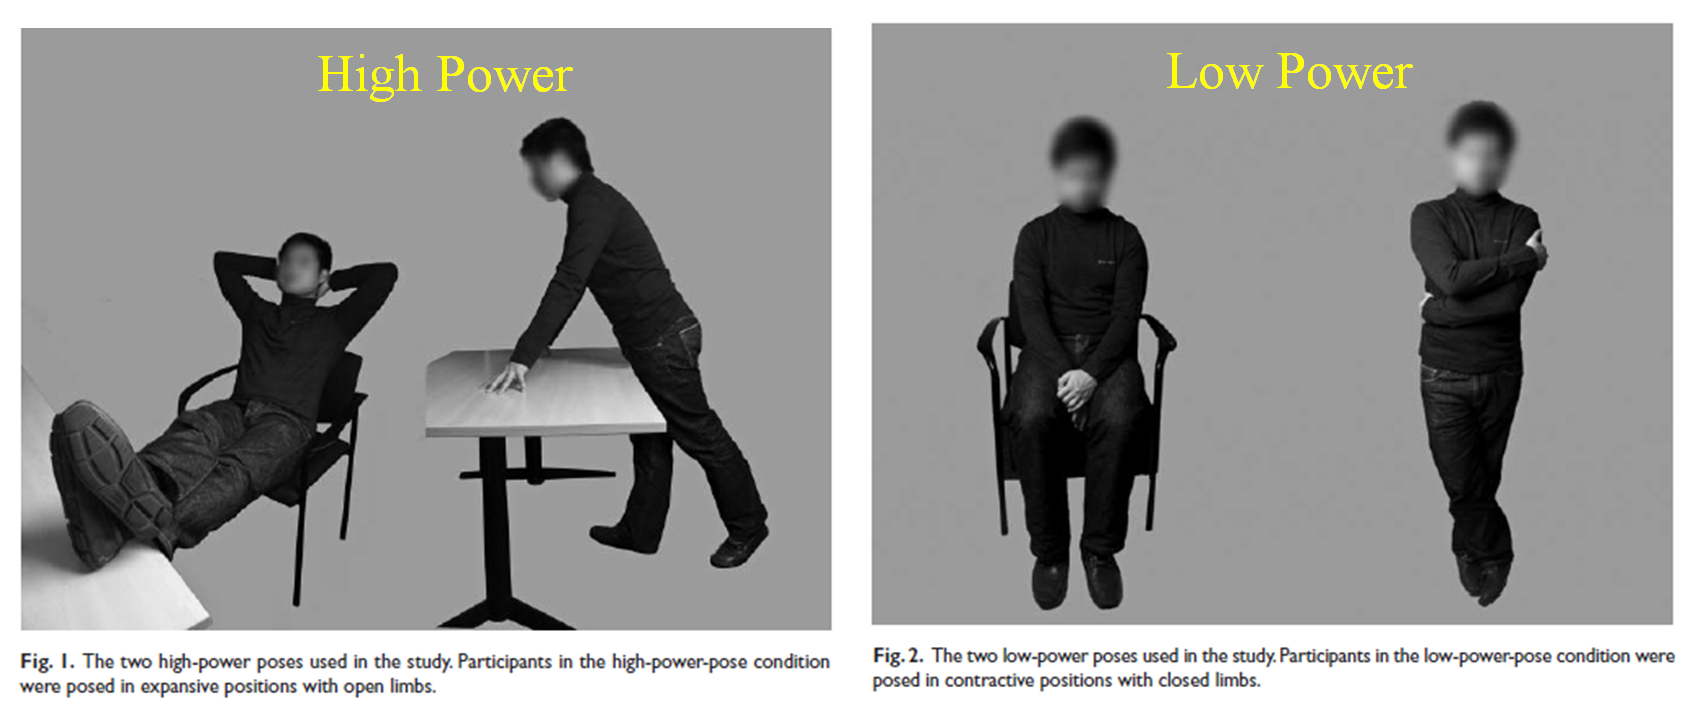
\includegraphics[width=\linewidth]{./images/2-posing}
  \caption{From Carney, Cuddy, and Yap (2010).}
  \label{fig:2-pose}
\end{figure*}

However, in 2015 a team of Eva Ranehill et. al \cite{ranehill2015assessing}
attempted to reproduce the results of the original 2010 experiment, using a
larger sample size of 200 persons. Their findings confirmed the subjective
experience of participants, but failed to find a significant effect on hormone
levels or risk taking. What followed was a flurry of additional replication
studies, which ultimately resulted in original author Dana Carney
\cite{carney2015} publically rescinding her belief in the physiological effects of
power posing.

This example illustrates a case of a \emph{failed replication}; the failure to find
the same results as an original study. One would hope that results could be
replicated, even under differing conditions. The failure to replicate a result
calls into question the original study's findings, though is not by itself a
conclusive refutation. For power posing, a collection of failed replications
undermines the original study, and \href{http://datacolada.org/37}{review of the existing literature}
\footnote{\url{http://datacolada.org/3}} points to publication bias as a reasonable
explanation for the existing successful replications.

It is important to note that, despite the evidence against power posing, it is
still impossible to conclusively say that no effect exists. It is possible that
the `true' effect is negative, or may be context-dependent. At best, we can say
that no strong evidence exists in favor of the physiological benefits of power
posing.

However, this example also raises some natural questions for the statistical
neophyte: ``What is a significant effect? How is significance determined? What
aspects of an experiment matter?'' These are the sorts of questions we shall
study below.

\section{Statistical Inference}
\label{sec:org03f2f4e}
Drawing quantitative conclusions from data is an exercise in \emph{statistical
inference}. \footnote{Formally, statistical inference involves determining parameters
of an underlying probability distribution. Choosing the \emph{correct} distribution
to describe the data is a key step in drawing reasonable conclusions.} For
example, we may be interested in education practice, and may want to know how
effective a new form of teaching might be; for example, we might believe that
getting students more involved via active participation in the classroom will
lead to better educational outcomes.\footnote{For instance: Active
learning.\cite{freeman2014active}} This change in practice is called a
\emph{treatment}.

In order to make an informed decision, we would want to know whether or not the
treatment is effective. To determine efficacy in reality, we would perform an
experiment, separating subjects into a group which receives the treatment or
into a \emph{control group} which does not,\footnote{The choice of control varies based on
application. In medical testing, it would be unethical to deny treatment to
those who are ill, so the standard practice in clinical trials is to compare a
new treatment against the best existing standard practice.} measure some desired
outcome with a quantitative metric, and perform data analysis to determine
significance. Explicitly, we have some measureable outcome \(Y_i\) for each
studied individual \(i=\nobreak1,\dots,n\), and postulate some model for the treatment,
such as

\begin{equation}\label{eq:model}
  Y_i = \mu + \beta x_i + \epsilon_i,
\end{equation}

where \(\mu\) is the average outcome without treatment, \(\beta\) is the amount the
outcome increases (or decreases!) with the treatment, \(x_i\) is one only for
those individuals \(i\) who received the treatment and zero otherwise, and
\(\epsilon_i\) is a noise term.\footnote{As engineers, our models tend to arise from
fundamental physical principles, such as conservation laws. For statisticians,
models often arise from simple compositions of probability distributions.
Statisticians do not \emph{literally} believe that effects are additive, but rather
make pragmatic choices that balance utility with analytic tractability. This
philosophy is embodied in the quote (attributed to George Box) ``All models are
wrong; some models are useful.''} We'll use this model as a running example
throughout this document.

In addition to our treatment, there may be some number of other variables at
play; for example, the prior knowledge students bring to a class, or
socioeconomic factors which help or hinder learning. We would want to control
these factors in order to draw a valid inference, usually through careful
\emph{experimental design}.

Finally, it is not enough to determine that a treatment works; we would like an
idea of how \emph{practically effective} treatment is, so that we can make informed
decisions about how to spend limited resources. If a particular treatment works,
but causes negligible changes in student learning, we might be better off
looking for a different approach, or just staying with the current best
practice.

\marginnote{Sidenote: Unlike engineers, statisticians draw a distinction between the terms
\emph{variable} and \emph{parameter}. Parameters are properties of a
distribution, while variables are (often random) measured quantities. Knowing
the difference may save you a headache when reading literature.}

We will elucidate these concepts below.
\subsection{Significance testing}
\label{sec:org2289415}
Testing for significance usually follows the framework of \emph{null hypothesis
significance testing} (NHST). The high-level philosophy of this framework is to
define a statistical model under the assumption that the treatment has no
effect. We then collect data, and check to see how compatible the data are with
this hypothesis. If the data are incompatible (in a precise statistical sense),
we reject the original assumption, and conclude that the treatment has some
effect.\footnote{This framework may seem a bit backwards at first. Proponents of NHST
note that the framework is in line with a \emph{falsificationist} perspective of
science, a philosphy of scientific practice advanced by Karl
Popper.\cite{popper2005logic} This is a somewhat controversial viewpoint, as the
null hypothesis is rarely advanced as a reasonable state of reality, and NHST is
often used to advance an alternative hypothesis rather than to falsify another.
However, NHST is certainly normative in social science, and from that
perspective alone is worth studying.}

In this framework, we must define a \emph{null hypothesis}, which defines a
statistical model under which the treatment confers no effect. For example, a
null hypothesis of zero effect in the model defined by \eqref{eq:model}
corresponds to \(\beta=0\). The null hypothesis may also include a statement about
the distribution of noise; it is common to assume the \(\epsilon_i\) are drawn
from a normal distribution with zero mean and (possibly unknown) variance
\(\epsilon_i\sim N(0,\sigma^2)\). \footnote{It is possible in some cases to get away
without assuming a particular distribution. This is called a \emph{nonparametric}
approach. Assuming a distribution in a \emph{parametric} approach often gives a
convenient mathematical form, and depending on the circumstances, can be robust
to departures from the underlying assumptions.}

Still working with \eqref{eq:model}, if we assume the null hypothesis,
we can manipulate the outcome variable to state

\begin{equation}\begin{aligned}
  Y_i &= \mu + \cancel{\beta}x_i + \epsilon_i, \\
      &\sim N(\mu,\sigma^2).
\end{aligned}\end{equation}

This is not a testable statement, though! We need a statement that involves the
treatment in some fashion. Let's separate the individuals that received the
treatment \(Y_i^t\) from those that did not \(Y_i^0\), and compute their averages

\begin{equation}\begin{aligned}
  \hat{Y}^t &= \frac{1}{n_t}\sum_{i=1}^{n_t} Y_i^t, \\
  \hat{Y}^c &= \frac{1}{n_c}\sum_{i=1}^{n_c} Y_i^c.
\end{aligned}\end{equation}

Under the null hypothesis, these are still normally distributed, with
\(\hat{Y}^t\sim N(\mu,\sigma^2/n_t)\) and \(\hat{Y}^c\sim
N(\mu,\sigma^2/n_c)\).\footnote{Taking an average reduces the variance; this is part
of why averaging is a useful operation.} Since these quantities share the same
mean, we may write

\begin{equation}\label{eq:contrast}
  \hat{Y}^t-\hat{Y}^c \sim N(0,\sigma^2(1/n_t+1/n_c)).
\end{equation}

\Cref{eq:contrast} provides \emph{testable} structure. If we collect data and find
that the observed difference is significantly non-zero, this will lead us to
reject the null hypothesis, and conclude that the treatment has some
effect.\footnote{Note that in \Cref{eq:contrast}, while we would probably like to see
a positive difference, a negative value is entirely possible!} Determining \emph{how
large} a difference is significant usually involves computing a \emph{p-value}.

\begin{figure}[!ht]
  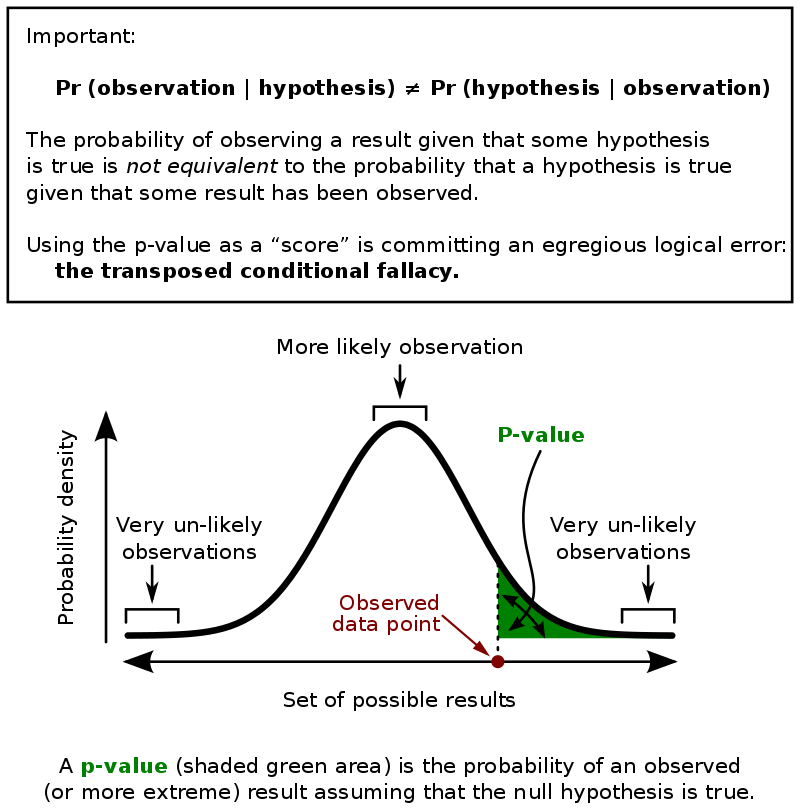
\includegraphics{./images/p-value}
  \caption{A very nice visual description from Wikipedia. This image
    depicts a \emph{one-sided} p-value. The two-sided case would consider
    the symmetric tail on the negative side of the distribution. In practice,
    one should always use the two-sided test when there exists the possibility
    of the effect being negative. The image text describes some additional
    logical fallacies involving p-values.}
  \label{fig:p-value}
\end{figure}

\subsection{The p-value}
\label{sec:org6f8c447}
The \emph{p-value} is a measure of how incompatible some data are with a given
hypothesis. It is a measure of surprise, and corresponds to the probability of
observing a result at least as extreme as what was observed. Figure
\ref{fig:p-value} visually depicts the p-value arising from a normal
distribution.

The p-value is used to determine \emph{statistical significance}; the smaller the
p-value, the less likely we were to find the observed results under the null
hypothesis. If the p-value arising from the data is smaller than some chosen
threshold, then we reject the null hypothesis. A standard \emph{significance
threshold} is \(5\%\); if \(p<0.05\), then we are said to reject the null hypothesis
at the \(5\%\) level.

\begin{figure}[!ht]
\begin{verbatim}
### P-value computation example
# Generates synthetic data, performs two-sample t-test
import numpy as np
from scipy.stats import ttest_ind
np.random.seed(0)                      # For reproducibility
# Define the ground truth
mu   = 0.0                             # Mean response
beta = 0.5                             # Treatment effect
sig  = 1.0                             # Noise standard deviation
# Define the sampling parameters
n = 100                                # Sample size
# Draw samples
Y_t = mu + beta + np.random.normal(loc=0,scale=sig,size=n) # Treatment
Y_0 = mu        + np.random.normal(loc=0,scale=sig,size=n) # Control
# Perform t-test
res = ttest_ind(Y_t,Y_0)        # Automates a two-sided t-test
pval = res[1]                   # Extract the p-value from results
# Report
print("pval = {0:}".format(pval))
# Recorded result
pval = 0.0011808425369
\end{verbatim}
\caption{Example code to simulate our model and run a t-test.}
\label{fig:p-value-computation}
\end{figure}

In our running example, we would compute a p-value from \eqref{eq:contrast}. If
\(\sigma\) were known exactly, we could do this easily from the normal
distribution. In practice, we rarely know \(\sigma\), so we use a \emph{t-test}
instead; this accounts for the additional randomness from having to estimate
\(\sigma\) from the data. Figure \ref{fig:p-value-computation} provides example
python code that generates some fake data under our simple model, and performs a
two-sample t-test on the resulting data.

Note that, despite the presence of large noise (\(\sigma=1.0\)) and a (relatively)
smaller effect (\(\beta=0.5\)), we obtain a rather small p-value of
\(p\approx10^{-3}\). This is largely due to our sample size; we happened to draw
enough samples such that we could cleanly discover the underlying effect. In
general, the more samples we draw, the more probable it is that we will find the
true effect (if it exists). The probability of rejecting the null hypothesis
when there exists a nonzero effect is called the \emph{power} of a test. Power is
typically hard to estimate, and is a complicated function of the effect size,
noise, and number of samples drawn.

The simple procedure above assumes certain properties of the noise \(\epsilon_i\).
If there is additional variability arising from other uncontrolled variables,
this may interfere with correct inference. For example, if the treatment is a
change in instructor approach, but only students of low socioeconomic status
took the control version of the class, then we would observe only a combination
of the treatment and socioeconomic effects -- this is called a \emph{confound}.
Standard practices from \emph{experimental design} are meant to address these issues.

\subsection{Balance and randomization}
\label{sec:orge2ee824}
\emph{Balance} is a property of an experimental design, and is important to help
ensure particular beneficial statistical properties.\footnote{Namely, a balanced
design will have higher statistical \emph{power} (probability of detecting a real
effect), and will help prevent \emph{heteroskedasticity} (unequal variability among
groups).} Suppose we are studying an education treatment, but we have 12
students in the control group and only six in the treatment (Fig.
\ref{fig:unbalanced}). With this sample, we have less information about the
treatment group. A \emph{balanced} design would place an equal number of students in
each group.

\begin{figure}[!ht]
  \centering
  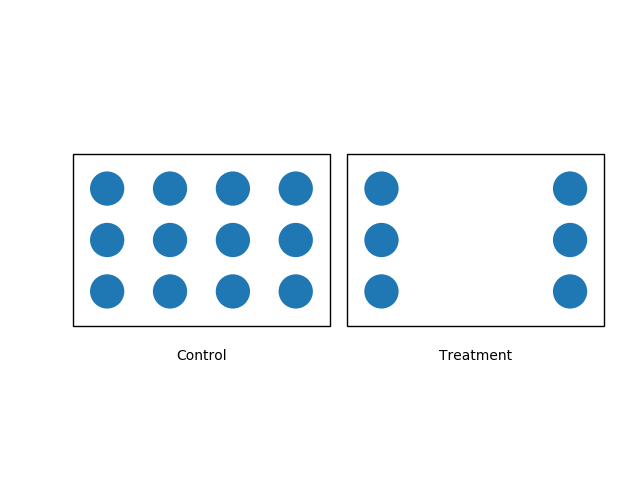
\includegraphics[width=0.85\textwidth]{images/balance}
  \caption{Example of an un-balanced design. Generally, we want the treatment
  and control to have the same number of subjects.}
  \label{fig:unbalanced}
\end{figure}

Other factors are not easy to measure or control. In an educational setting,
prior knowledge of a student can be difficult to measure, and socioeconomic
status may be challenging to determine. In practice, we balance the variables
that we are aware of, and \emph{randomize} the remaining samples. On average,
randomization takes care of any confounding variables we did not explicitly
control (Fig. \ref{fig:randomize}). It is standard practice to randomize a
design, and you should be highly suspicious of an experiment which does not
randomize! Figure \ref{fig:randomize} illustrates the importance of randomizing
an experiment through a somewhat cartoonish example.

\begin{figure*}[!ht]
  \centering
  \begin{minipage}{0.45\textwidth}
    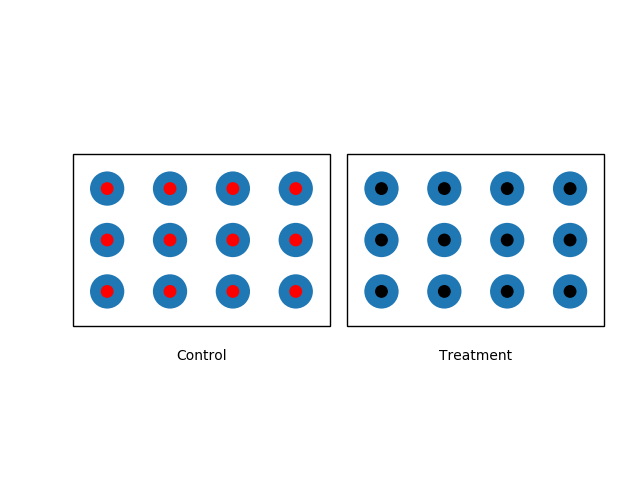
\includegraphics[width=1.05\textwidth]{images/nonrandom}
  \end{minipage} %
  \begin{minipage}{0.45\textwidth}
    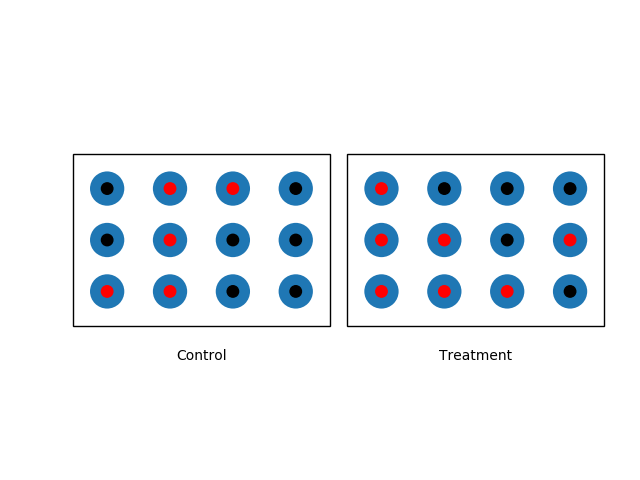
\includegraphics[width=1.05\textwidth]{images/random}
  \end{minipage} %
  \caption{Suppose we have selected students from two different schools to
  take part in an educational study, and are bringing 12 students from each
  school to our lab. The schools are identical in terms of demographics,
  socioeconomic status, and other factors, so for simplicity's sake we
  place all the students from one school in the control, and the other
  school in the treatment group (Left image). However, though a bit of
  miscommunication, we are unaware that one school is a 10 minute walk away
  from our lab, while the other lies 5 hours away. The students from the
  distant school rode a bus all night to take place in this exciting
  study, and are extremely tired. This effect will confound the results
  of the experiment! Had we been aware of this issue, we could have manually
  balanced. However, had we randomized the design (Right image), this issue
  would have been handled of automatically. Randomization helps to
  deal with issues of which we are not aware.}
  \label{fig:randomize}
\end{figure*}

\subsection{Practical vs statistical significance}
\label{sec:orgf5094ed}
When making a decision, it is not enough to consider statistical significance.
Even if the effect size is vanishingly small, it is still possible to find a
significant p-value by drawing enough samples. Thus, it is important to consider
\emph{practical significance} when deciding on the efficacy of a treatment.

There are various measures of practical significance. One may directly consider
the estimated effect size; in our example, this would be
\(\hat{\beta}=\hat{Y}^t-\hat{Y}^0\) estimated from the data. There is also
\emph{Cohen's d}, a normalized version of the effect size. With our model notation,
\(d\) is defined by

\begin{equation}\label{eq:cohen}
  d = \frac{\hat{Y}^t-\hat{Y}^0}{s},
\end{equation}

where \(s\) is the estimated standard deviation. Cohen's \(d\) is useful when there
are no meaningful units for the measured response, and there exist standardized
values for judging the size of \(d\).
\subsection{And so on}
\label{sec:org196b26b}
There are many more important aspects of statistical inference, and what I've
covered has been at a rather high level. Rather than get too lost in the weeds,
let's move on to how learning from people can fail, and talk about the
\emph{replication crisis}.

\section{Issues with Sigificance Testing}
\label{sec:org67dae6b}
We've seen some of the machinery of null hypothesis significance testing: How we
can draw particular kinds of conclusions from data, and a bit about how to
design experiments. If these techniques are well-founded, why is there a
reproducibility crisis? In this section, we'll explore some plausible reasons.

\subsection{P-hacking}
\label{sec:org642b5c9}
A dirty secret of scientific literature is that papers containing statistically
significant results are more likely to be published. This is known as
\href{https://en.wikipedia.org/wiki/Publication\_bias}{publication bias},\footnote{\url{https://en.wikipedia.org/wiki/Publication\_bias}} and leads
to a number of unfortunate effects. One of these effects is on research practice
itself -- the desire to publish incentivizes obtaining statistical significance,
and adjusts researcher behavior, whether consciously or not.

P-hacking is the practice of \href{https://fivethirtyeight.com/features/science-isnt-broken/\#part1}{modifying a data analysis}
\footnote{\url{https://fivethirtyeight.com/features/science-isnt-broken/\#part1}} in order
to obtain an acceptably low p-value. There are many ways to accomplish this. One
method is called \emph{multiple hypothesis testing}.

\subsection{Multiple hypotheses testing}
\label{sec:org298a165}
Remember the Dungeons and Dragons analogy above? D\&D is played by rolling dice
many times -- eventually, someone will roll a twenty, and succeed where they
would otherwise fail. The \emph{multiple hypothesis testing} pathology works much the
same way: A hapless (or unscrupulous!) researcher decides to measure many
different responses from the same subjects, and reports only those results which
are statistically significant. Even if no effect exists, since we are forced to
measure in the presence of noise, there is a small chance (\(5\%\) for \(p<0.05\))
for each hypothesis to come up significant. Falsely rejecting the null
hypothesis is called making a \emph{false discovery}, and does not result in real
scientific progress.\footnote{If we test \(100\) independent hypotheses at the \(5\%\)
level, there is a \(0.6\%\) chance that we will \emph{not} make a false discovery. If
we're trying to avoid false discoveries, that's quite bad!}

As an example, suppose a researcher seeks to determine whether there is a link
between Skittles and cancer. The researcher finds no effect for Skittles in
general, so decides to study the effects of particular \emph{flavors} of
Skittles.\footnote{There are \emph{a lot} of flavors of Skittles.} Finally, after
testing all possible flavors, the researcher finds a statistically significant
link between Liquorice Aniseed\footnote{Apparently a British thing.} Skittles and
cancer, and publishes the results, not noting that multiple hypotheses were
tested to arrive at the given conclusion.

One of the big issues here is communication. If all authors noted how many
hypotheses they tested to arrive at statistically significant results, we could
adjust our expectations accordingly. However, one can give a false impression
by selectively reporting analysis and results.

\subsection{Sample sizes}
\label{sec:org7d0bc30}
One challenge with studying people is variability. Noise tends to be
comparatively tame in experiments involving the physical world; physicists tend
to use a \(5\sigma\) criteria for discovery, which corresponds to
\(p\lesssim5\times10^{-7}\).\cite{demortier2007p} Such a stringent significance
criterion is only possible through careful control of variability, which is
simply not possible in most social experiments. Drawing more samples (e.g.
studying more people) helps to lessen the effects of noise, but still probably
won't get us to \(p<10^{-7}\) in social experiments!

The quantity to control when designing a study is (statistical) \emph{power}\footnote{The
power of statistics is completely different from that of physics; statistical
power is dimensionless.}: The probability of rejecting the null hypothesis,
\emph{given that the null is false}. Power is a function of the significance
threshold (\(p<p_c\)), the effect size (\(\beta/\sigma\) in the model above), and
the sample size.\footnote{Power also depends on a lot of other factors: The analysis
used, the particular test statistic chosen, and possibly more stuff.} The
significance threshold is usually chosen to be \(p_c=0.05\), and an acceptably
high power is considered to be \(P=0.80\). This leaves the effect size
\(\beta/\sigma\) as an unknown, and the sample size \(n\) as a chooseable
quantity.

Determining the required sample size \(n\) for the desired power requires making a
guess at the effect size! This is challenging to do well. If a researcher is
overly optimistic about the effect size, they may unknowingly select a sample
size which is too small, leading to a low power study. Low power studies
introduce new kinds of issues.

\subsection{Type S / Type M errors}
\label{sec:org419301d}
Classical NHST considers two kinds of error: Type I error is the probability of
\emph{falsely rejecting} the null hypothesis,\footnote{There's a related, but different,
concept called a \emph{false discovery rate} (FDR). You can think of the false
discovery rate as being related to multiple hypothesis testing, and there are
procedures which are designed to control the FDR.} while Type II error is the
probability of \emph{failing to reject} the null hypothesis when it is
false.\footnote{Type II error is the complement of the statistical power; that is
\(P=1-Err_{II}\)} Authors Andrew Gelman and John Carlin \cite{gelman2014beyond}
introduced Type S (Sign) and Type M (Magnitude) errors, which can be rather
dramatic in low-power settings (Fig. \ref{fig:power006}).

\begin{figure*}[!ht]
  \centering
  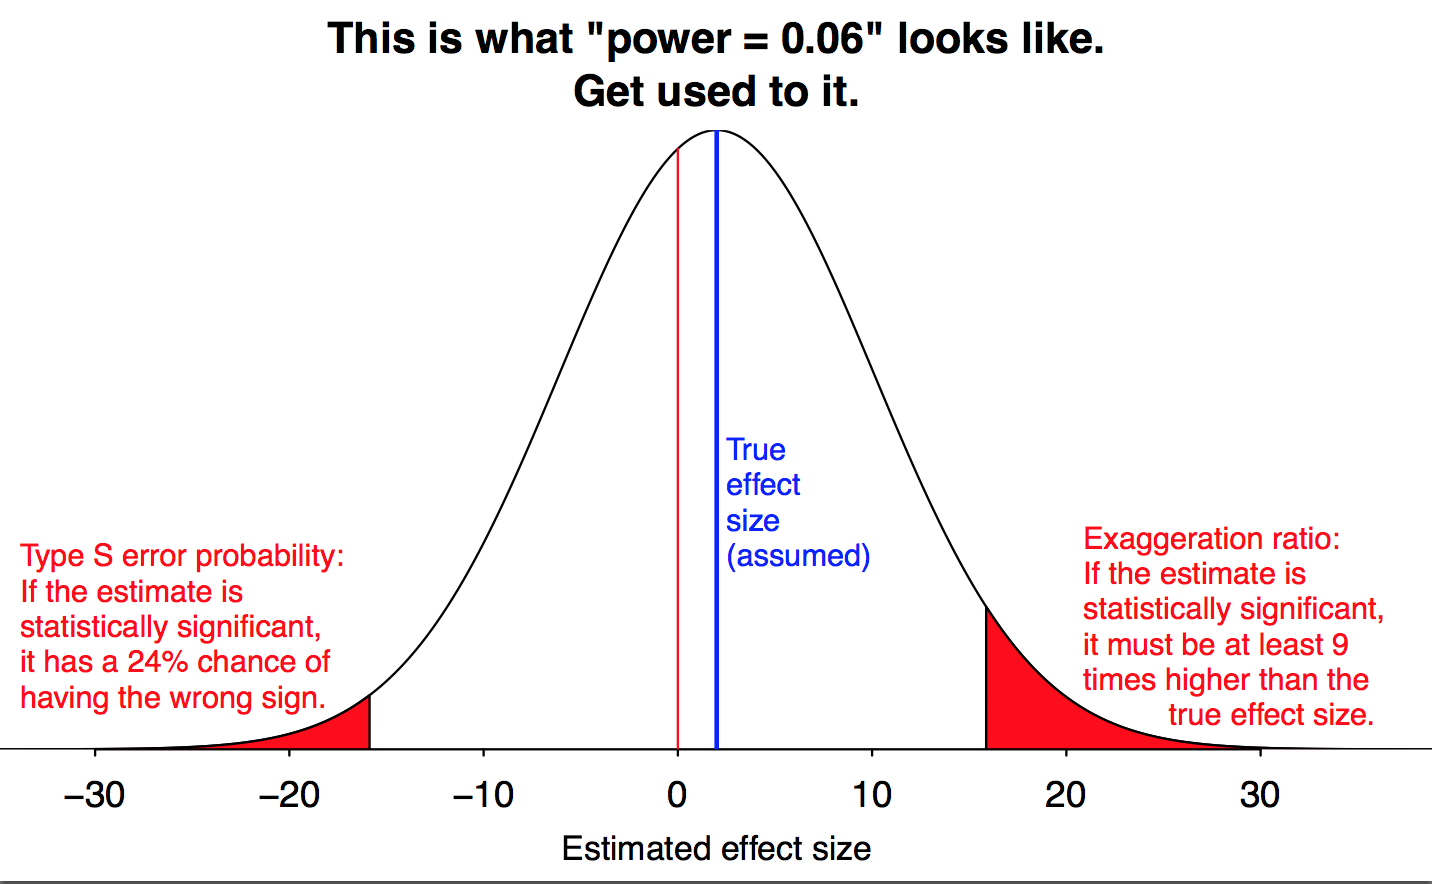
\includegraphics[width=0.65\textwidth]{images/power006}
  \caption{Graphic prepared by Andrew Gelman to illustrate the dangers of low
  power ($P=0.06$) studies. In this case, }
  \label{fig:power006}
\end{figure*}

Type S error is the probability of \emph{incorrectly estimating the sign of an
effect}. When studying a treatment, we would probably like to know whether or
not it helps or harms. It is possible in noisy settings that we may conclude a
treatment is beneficial, \emph{when in reality it is harmful}, or vise versa. Type S
error measures how likely we are to make this mistake.

Type M error is also called the \emph{exaggeration ratio}, and is the minimum factor
by which we must over-estimate the effect size, in order to reach statistical
significance. Figure \ref{fig:power006} illustrates this issue well: In the case
where noise drowns out the effect, any statistically significant results we may
find will \emph{necessarily} over-estimate the true effect.

These sorts of issues chip away at our confidence in published literature. For
low-powered studies, the published results may claim that a particular treatment
is beneficial, when in reality it actually harms. In the event that a treatment
actually is beneficial, it is quite possible the intervention is substantially
less effective than the results may suggest. Gelman and Carlin actually
recommend framing study design in terms of Type S and M error, rather than the
traditional power design.

\section{Recommendations}
\label{sec:orgcbf2fd0}
Given these issues, you may be feeling concerned. For those of us that would
like to make practical choices based on studies involving humans (e.g.
educators), this is particularly alarming -- How can we make informed decisions
if \href{http://journals.plos.org/plosmedicine/article?id=10.1371/journal.pmed.0020124}{most published research findings are false}?\cite{ioannidis2005most} I've got
some practical recommendations below which will (hopefully) help.

\subsection{Reading literature}
\label{sec:orgc35c2cd}
\begin{enumerate}
\item Practice skeptical reading:
\label{sec:orga55366b}
When reading about findings regarding human beings, whether from psychology,
medicine, or dietary advice, treat findings with skepticism. A great place to
practice this skeptical reading is in science journalism. Science journalists
are often not trained in statical techniques, and lack the time, incentives, or
tools to properly evaluate the work they report on. Therefore, it's a good idea
to read press releases and news articles on new fad diets or surprising
psychology studies with a healthy bit of skepticism.

This practice is particularly important for \emph{effects you are personally inclined
to believe}. For example, much research on \emph{stereotype threat} has been carried
out at Stanford, and members of the Stanford community may be inclined to have a
favorable outlook towards this research.\cite{spencer1999stereotype} However,
meta-reviews \cite{flore2015does} of the literature point to signs of publication
bias; given our discussion of Type M errors above, this suggests the effects of
stereotype threat may be over-estimated.

If that sentence makes you angry, please calm down! I'm not saying stereotype
threat doesn't exist. I'm saying that \emph{studying people is inherently difficult,
and so our knowledge of the human experience is imperfect}.

There's a relevant quote from the Open Science Collaboration which I really
like: "An ideological response would discount the arguments, discredit the
sources, and proceed merrily along. The scientific process is not ideological.
Science does not always provide comfort for what we wish to be; it confronts us
with what is."\cite{open2015estimating} Our aim in doing science is \emph{not} to
confirm what we already believe. It is to discover how the universe operates, in
reality. Sometimes that means being wrong.

This leads into my next recommendation:

\item Get comfortable with uncertainty:
\label{sec:orgbacddb0}
Studying humans is inherently uncertain and challenging, so it's best to get
used to that fact. Expecting to be able to find \(p<10^{-7}\) in a social
experiment is patently absurd, but so is pretending to have certainty about the
human condition. Rather than thinking or saying ``the research shows X'', it's
better to state ``the research \emph{suggests} X''. The difference is subtle, but
important. Internalizing this difference, and being able to distinguish between
degrees of uncertainty, is important for working in high-noise environments.

\item Compare relevant effect sizes:
\label{sec:orga74595a}
This one is a very practical (though not always applicable) technique: Compare
published effect estimates with similar effects. For example, if a treatment
purports to add as many years to your life as quitting smoking, that's a
\emph{literally incredible} claim! Building a bit of knowledge about relevant effects
is useful for orienting yourself in the literature, and is positively necessary
if you wish to become well-versed in a subject.
\end{enumerate}

\subsection{In practice}
\label{sec:org41b0bc8}
\begin{enumerate}
\item Get solid statistical training:
\label{sec:orge90a6b5}
This should come as no surprise, but if you want to do social science in
practice, you should get some serious statistical training. Take classes, and
gain some serious statistical background before attempting to study human
behavior.
\item Avoid low power designs:
\label{sec:org80b1809}
Even once you have some statistical background, avoid falling into low power
experimental designs. One practice when doing power calculations is to set
effect sizes aspirationally high, the idea being that, if the real effect is
smaller than guessed or than some practical threshold, the study will simply

suggest you might find the wrong sign, or grossly overestimate the effect. If
you suspect you are studying a small effect, either design the study accounting
for that, or seriously question whether studying the effect is worthwhile at
all.
\item Preregister studies and establish pre-analysis plans:
\label{sec:org1a43850}
\href{https://www.psychologicalscience.org/observer/research-preregistration-101}{Preregistration}
\footnote{\url{https://www.psychologicalscience.org/observer/research-preregistration-101}}
is  a practice  meant  to  help prevent  p-hacking;  it  involves detailing  and
publishing an analysis plan \emph{before the experimenter carries out the study}. One
could perform some exploratory data analysis, determine what to test, detail the
experimental and  analysis plan, and then  carry out the plan  according to what
was publically stated. If the authors stick  to the plan, then the reader can be
confident  that particular  decisions  were  made not  in  order  to p-hack  the
results, but rather were made before the data were ever seen.
\end{enumerate}
\subsection{Further Reading}
\label{sec:org0a6530b}
The replication crisis (or at least some of the underlying issues) have been
around for a very long time. \href{http://calteches.library.caltech.edu/51/2/CargoCult.htm}{Richard Feynman} gave a commencement speech at
CalTech back in the day warning about similar issues. More recently, \href{https://www.youtube.com/watch?v=J5A5o9I7rnA\&list=WL\&index=21}{Laura
Arnold} gave a TEDx talk on the replication crisis -- she's a philanthropist, and
is personally invested in drawing proper inferences from data to make informed
decisions.

If you're serious about learning more about the nuts and bolts of statistics as
it pertains to social science and the replication crisis, I have some
recommended reading for you. The blogs of \href{http://andrewgelman.com/}{Andrew Gelman}
\footnote{\url{http://andrewgelman.com/}} and \href{http://datacolada.org/}{Leif Nelson} \footnote{\url{http://datacolada.org/}}
provide lucid, often less-technical perspective on current statistical issues.
I've drawn from them for these notes. The website \href{http://callingbullshit.org/syllabus.html}{callingbullshit} attacks
similar issues, but with a somewhat broader perspective.

That being said, the best place to start with statistics is at the very basics;
consider taking an introductory statistics course if you've never seen the
material before. There's a lot of important concepts I didn't cover in this
document.

\section{Acknowledgements}
\label{sec:org6006a20}
I'd like to thank John Arakaki for helpful comments on an early version of these
notes.

\bibliographystyle{plain}
\bibliography{bibtex_database}

\section{Appendix}
\label{sec:org5a81e8e}
\end{document}
